
\ifsupershortmlslda

\else

\frame {

\frametitle{Problem}

\begin{itemize}
	\item We have documents in multiple languages
	\item They are annotated with the same {\bf continuous response}
	\begin{itemize}
		\item Rating of a product
		\item Movie review
		\item Percentage of people who retweet a tweet
                \item Percentage of people consider a comment ``extreme''
	\end{itemize}
	\item Can learning a model in multiple languages at once help?

	\pause

	\begin{block}{}
		For languages where you don't have many resources, {\bf yes!}
	\end{block}

\end{itemize}

}

\begin{frame}[t]{Conceptual Approach}

  \only<1>{
\includegraphics[width=0.85\linewidth]{mlslda/text_topics_prediction_0}}
  \only<2>{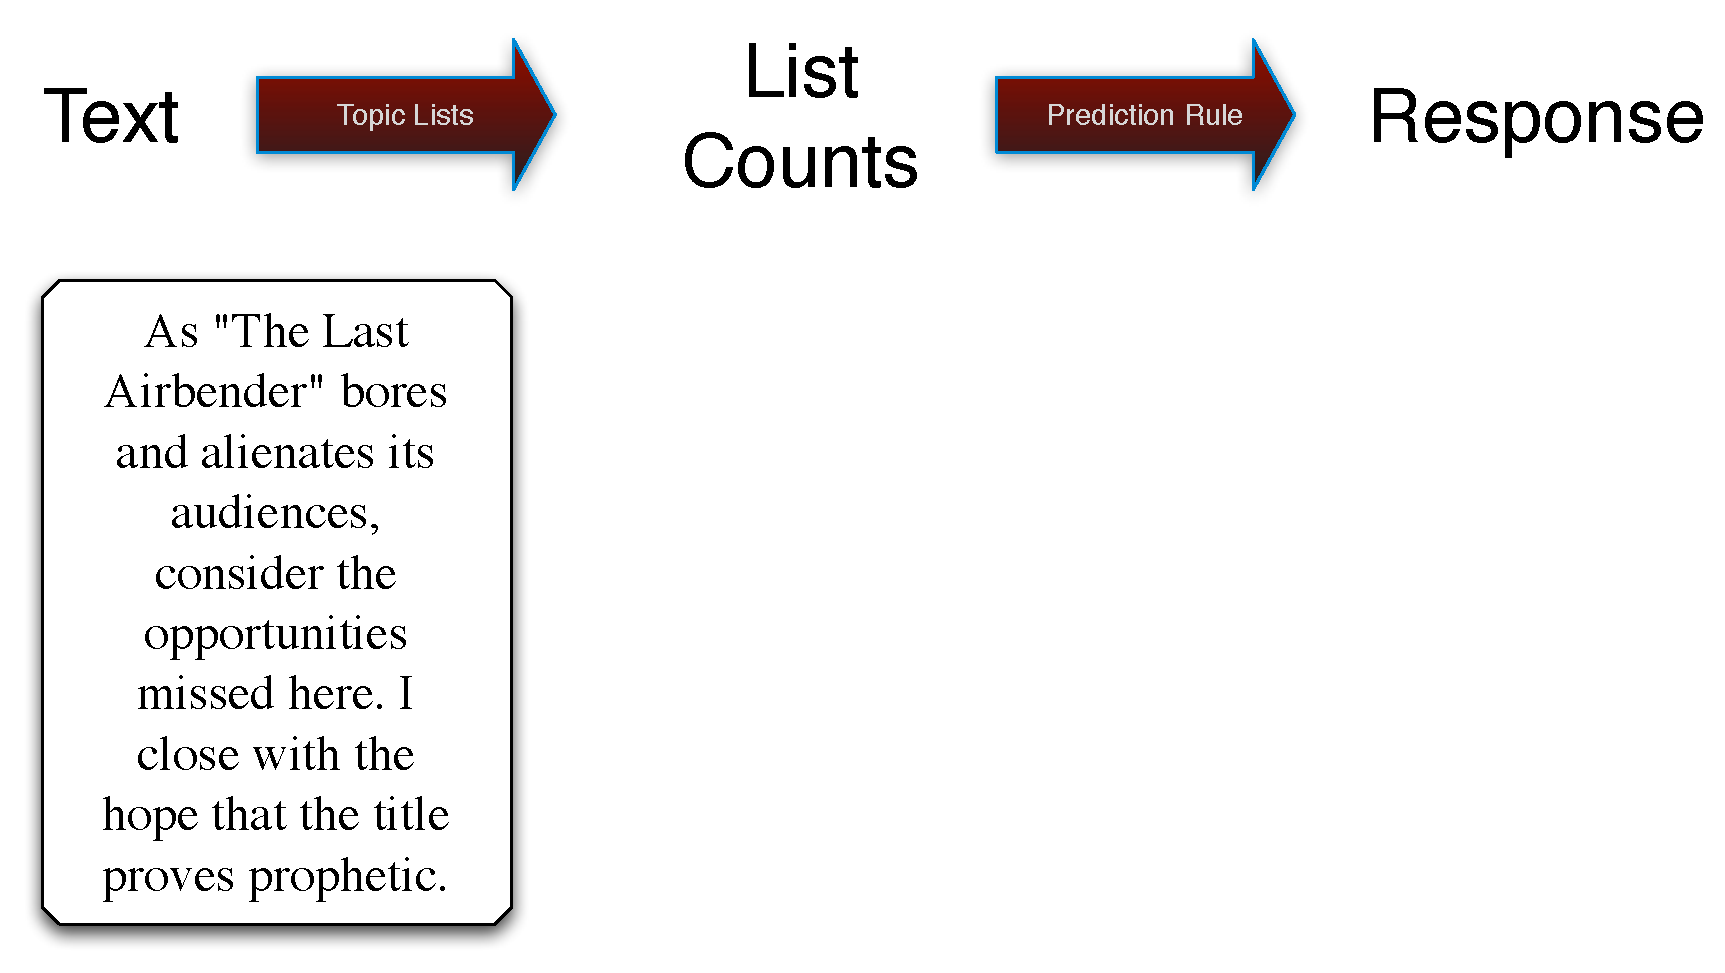
\includegraphics[width=0.85\linewidth]{mlslda/text_topics_prediction_1}}
  \only<3>{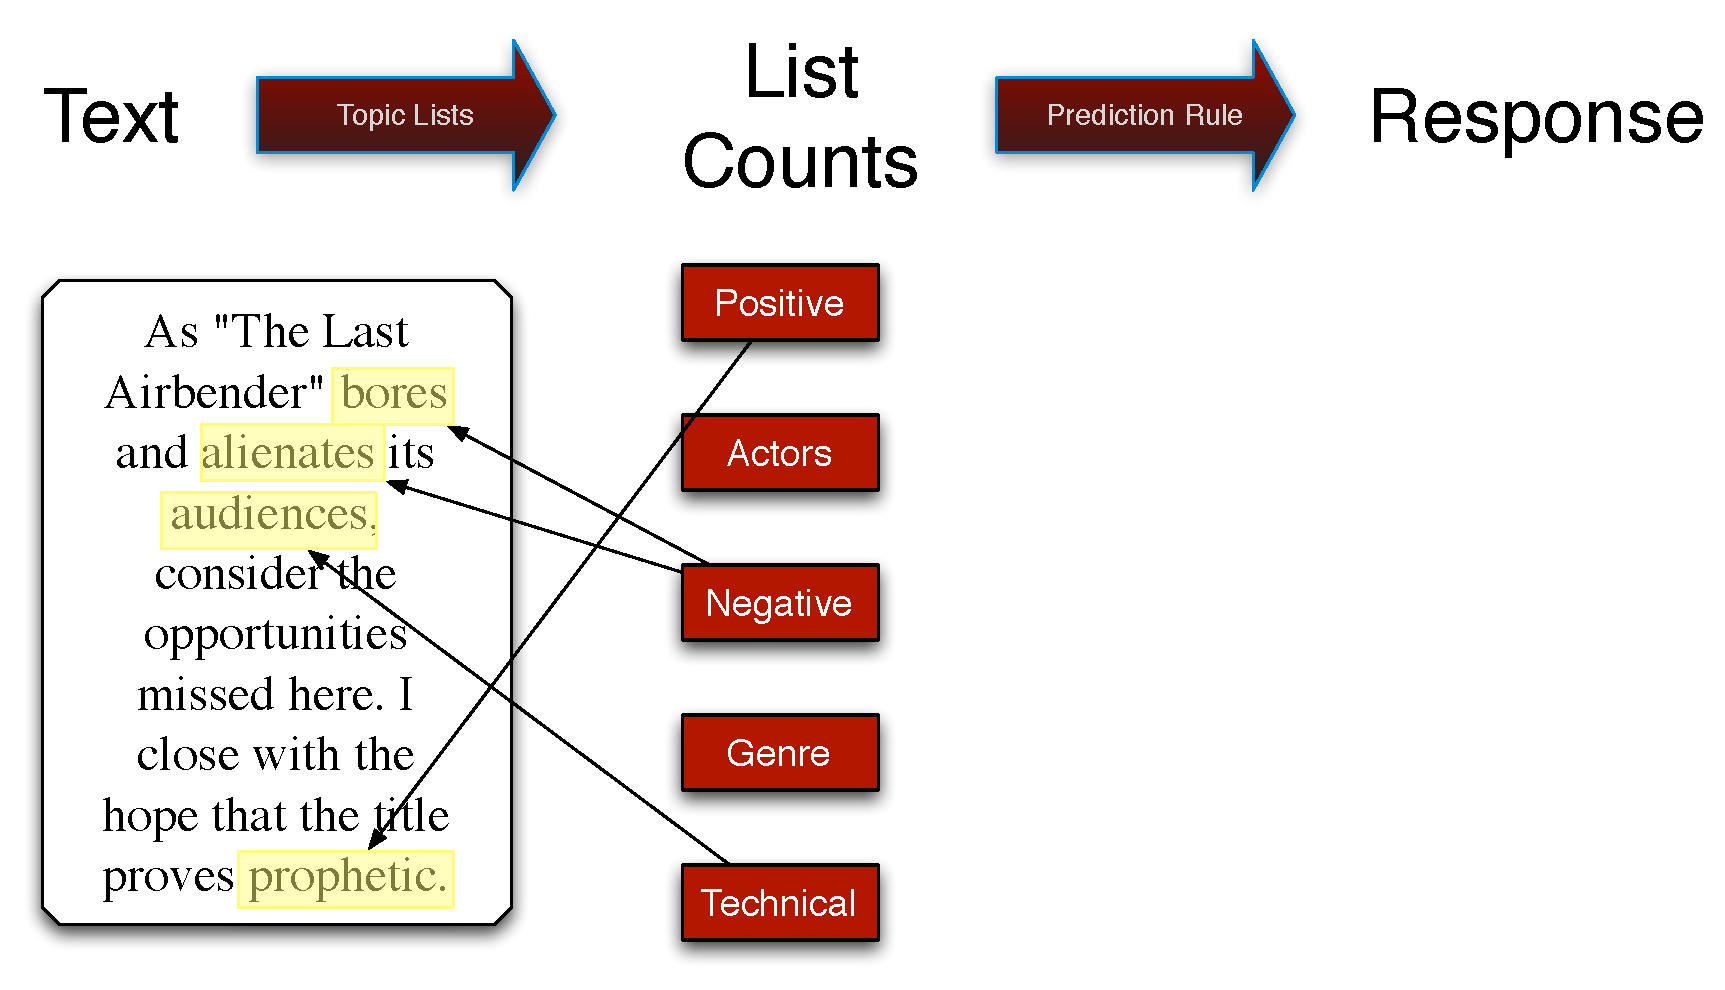
\includegraphics[width=0.85\linewidth]{mlslda/text_topics_prediction_2}}
  \only<4>{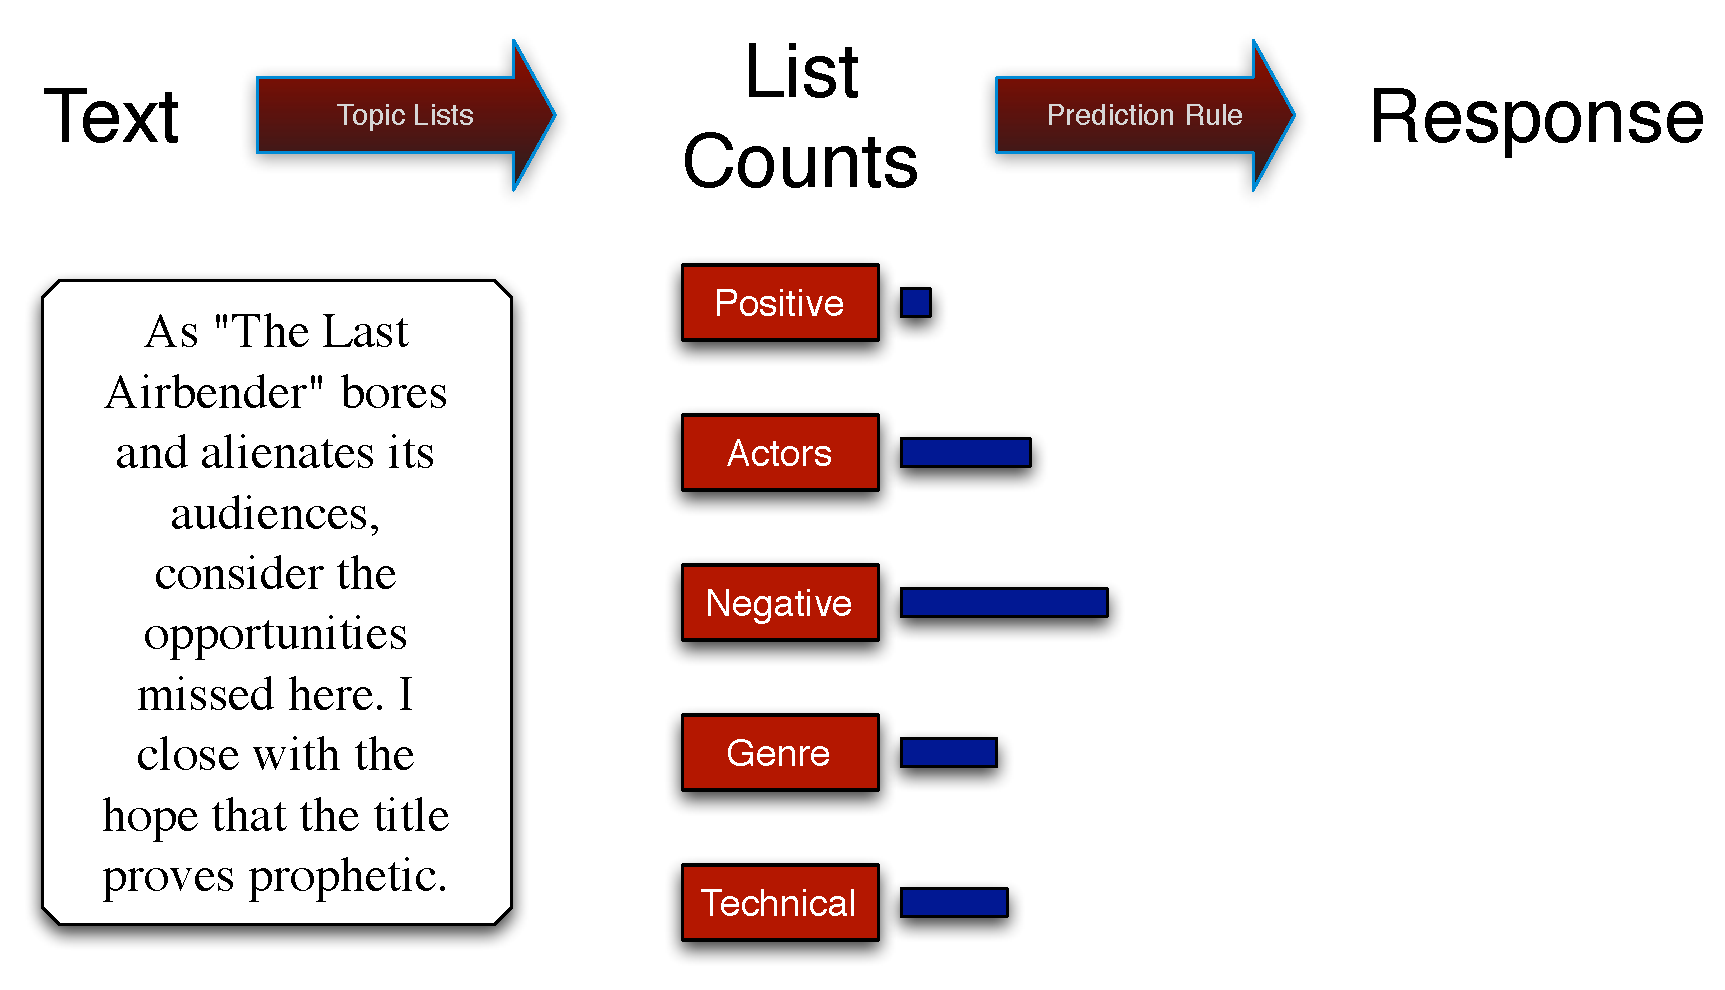
\includegraphics[width=0.85\linewidth]{mlslda/text_topics_prediction_3}}
  \only<5>{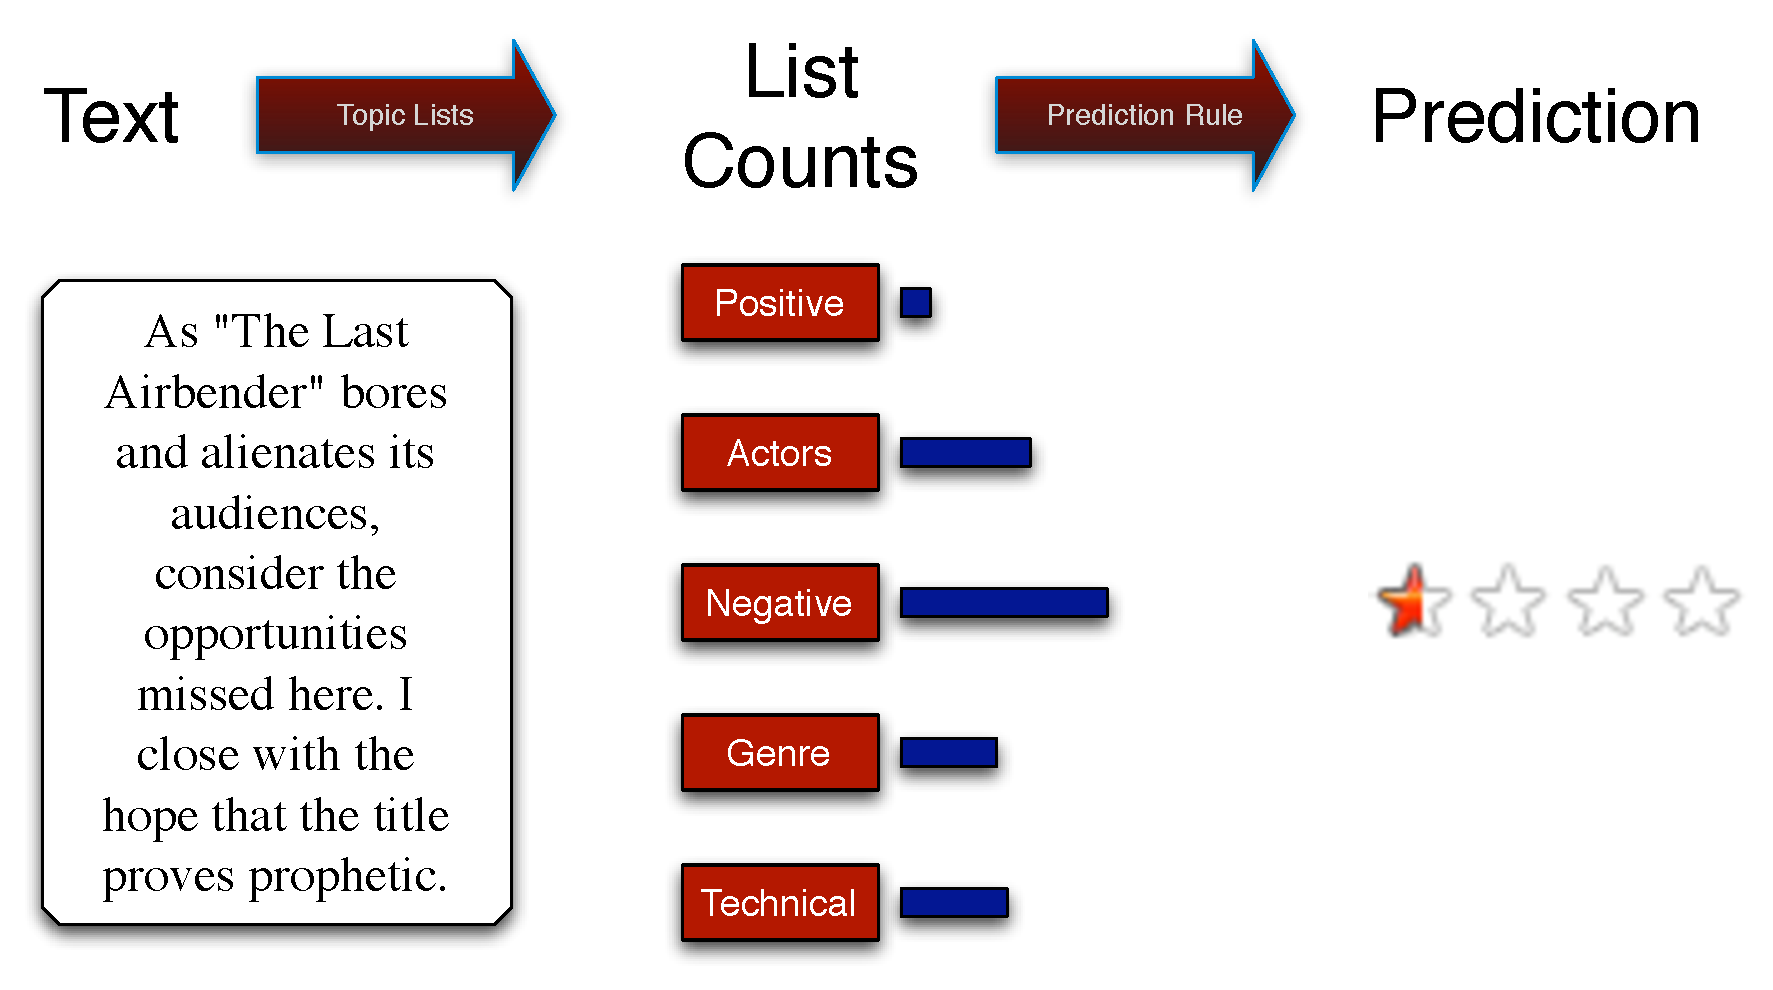
\includegraphics[width=0.85\linewidth]{mlslda/text_topics_prediction_4}}
  \only<6>{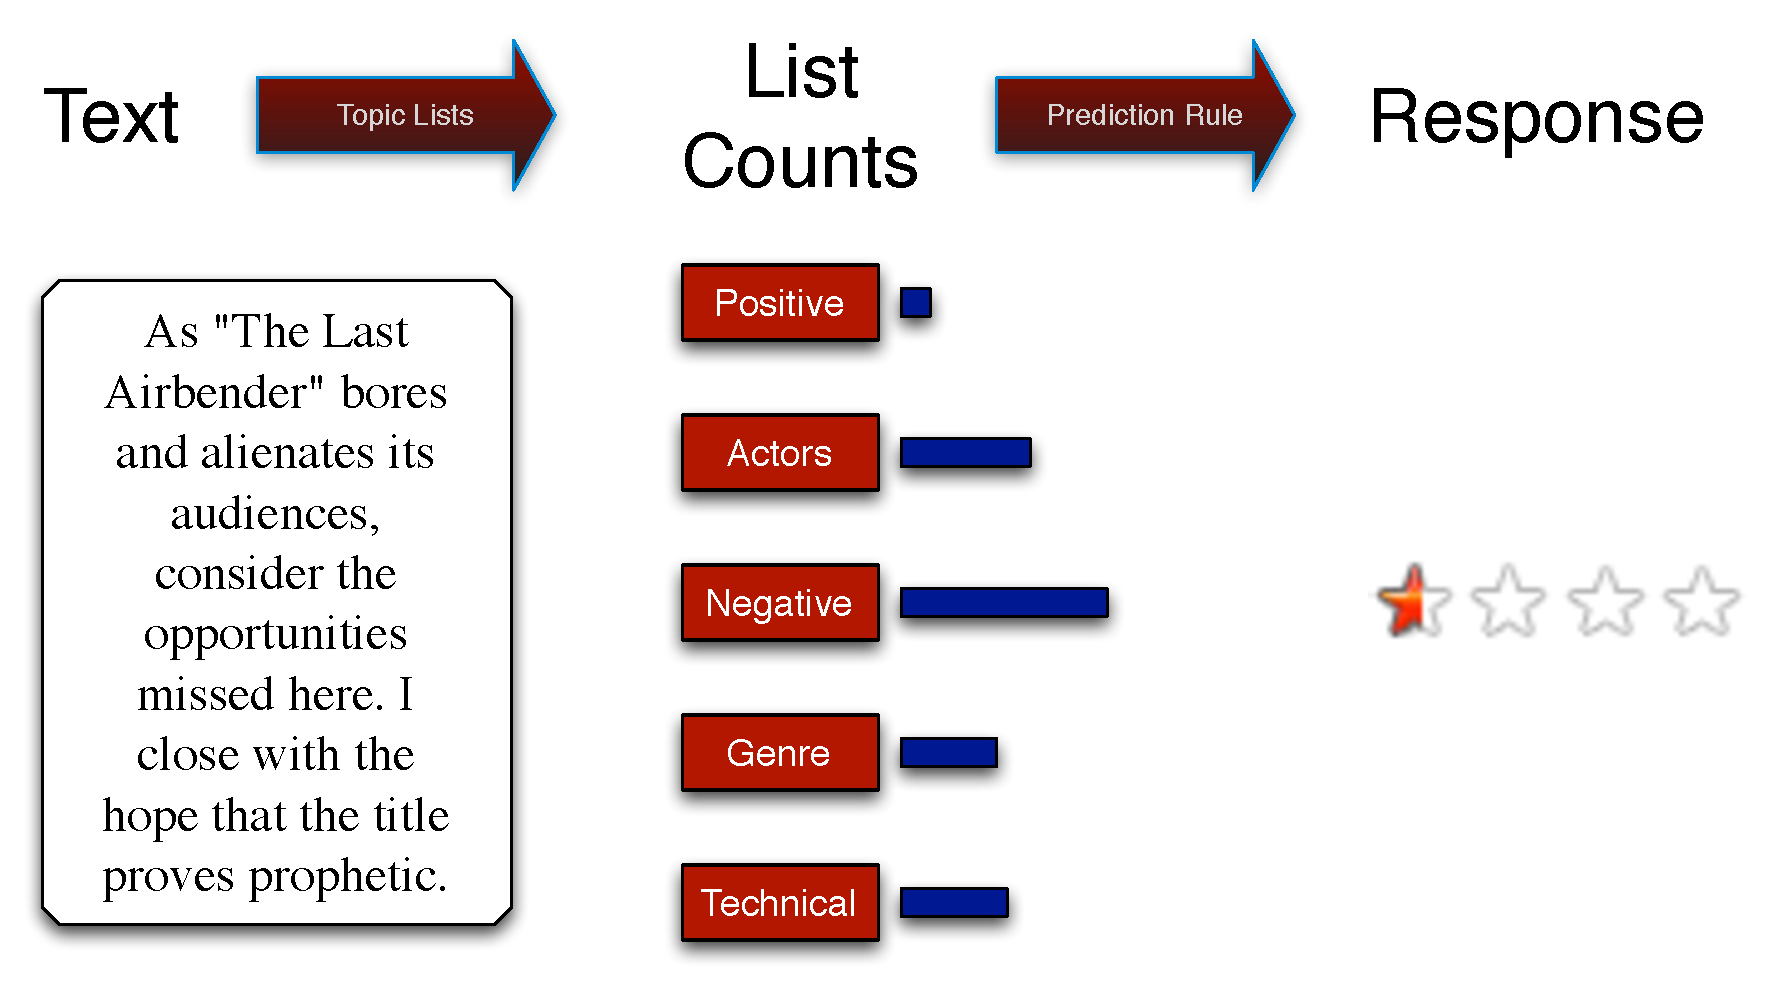
\includegraphics[width=0.85\linewidth]{mlslda/text_topics_prediction_5}}
  \only<7>{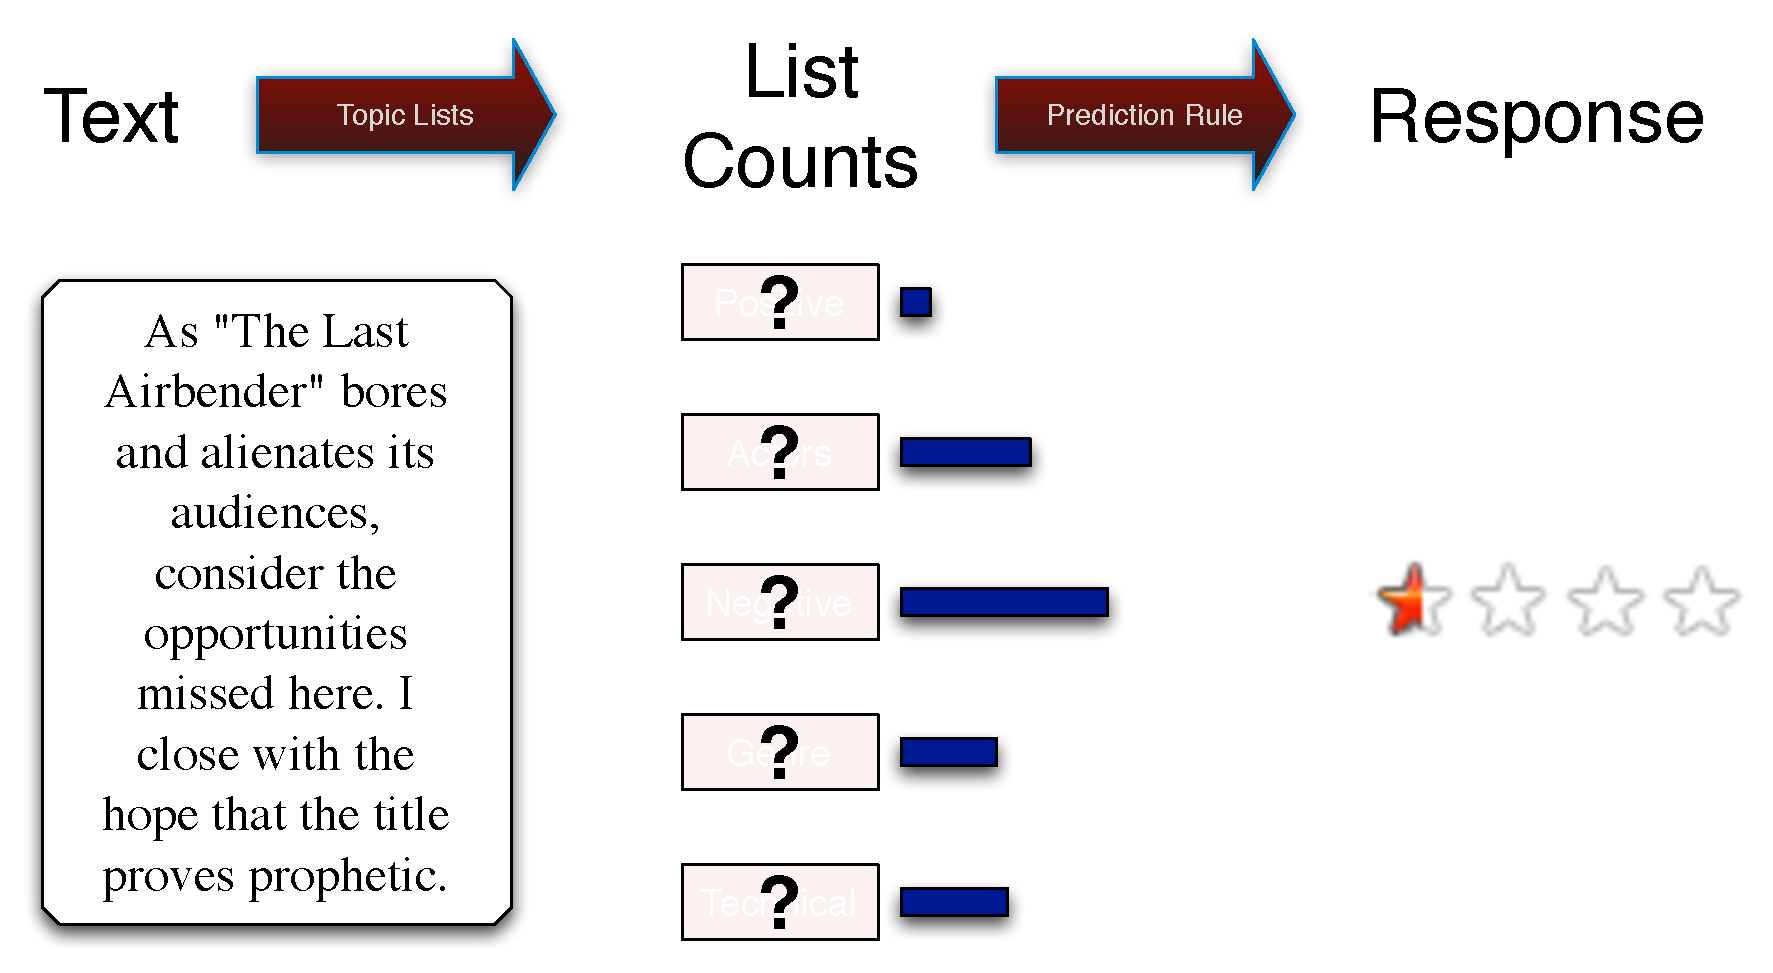
\includegraphics[width=0.85\linewidth]{mlslda/text_topics_prediction_6}}

  \only<5>{
  	\begin{center}
		Similar to social science methodology LIWC~\cite{pennebaker-99}
	\end{center}
  }

  \only<6>{
    \begin{itemize}
      \item {\bf Assumption:} We can create list counts from documents in any language
      \item {\bf Observation:} Once we have list counts, underlying language doesn't matter
    \end{itemize}
  }

  \only<7>{
  	\begin{block}{}
		\begin{center}
		What if we don't know the lists?
		\end{center}
	\end{block}
  }

\end{frame}

\iftmreview

\begin{frame}{Putting Pieces Together}

	\begin{itemize}
	\item How do we learn the word lists?
	\begin{itemize}
		\invisible<-2>{  \item Topic Models }
	\end{itemize}


	\item How do ensure that the word lists reflect sentiment?
	\begin{itemize}
		\invisible<-3>{  \item Supervised Topic Models }
	\end{itemize}

	\item How do make the word lists make sense across languages?
	\begin{itemize}
		\invisible<-4>{  \item Semantic Resources } \visible<5>{ }
	\end{itemize}
	\end{itemize}
\end{frame}



\providecommand{\graphscale}{0.6}


\newcommand{\dirfunc}[3]{ \frac{ \prod_{#1}^{#2} \g{ #3 } } { \g{ \sum_{#1}^{#2} #3 }}}
\newcommand{\dirnum}[4]{ \frac{\g{ #3 }}{#4} \prod_{#1}^{#2} }
\newcommand{\dirden}[3]{ \g{ \sum_{#1}^{#2} #3 } }

\section{Topic Model Introduction}

\begin{frame}

	\frametitle{Why topic models?}

	\begin{columns}

	\column{.3\linewidth}

	
\includegraphics[width=1\linewidth]{topic_models/newspapers}

	\column{.55\linewidth}

	\begin{itemize}
		\item Suppose you have a huge number of documents
		\item Want to know what's going on
		\item Can't read them all (e.g. every New York Times article from the 90's)
		\item Topic models offer a way to get a corpus-level view of major themes
		\pause
		\item Unsupervised
	\end{itemize}


	\end{columns}

\end{frame}

\frame{
\begin{center}
\frametitle{Conceptual Approach}
From an \textbf<1>{input corpus} and number of topics \textbf<1>{$K$} $\rightarrow$ \textbf<2>{words to topics} \\
\only<1>{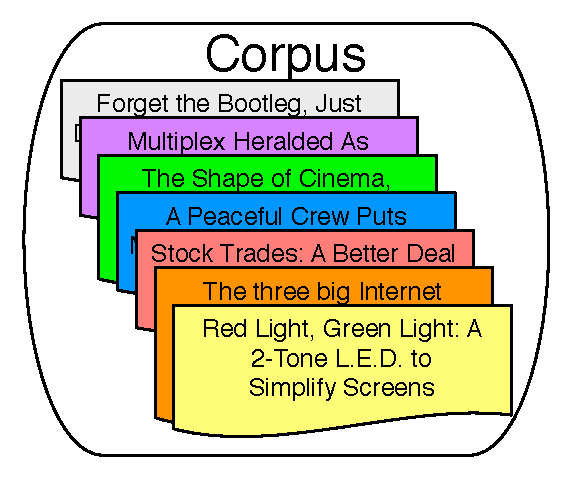
\includegraphics[width=0.6\linewidth]{reading_tea_leaves/figures/heldout_0} }
\only<2>{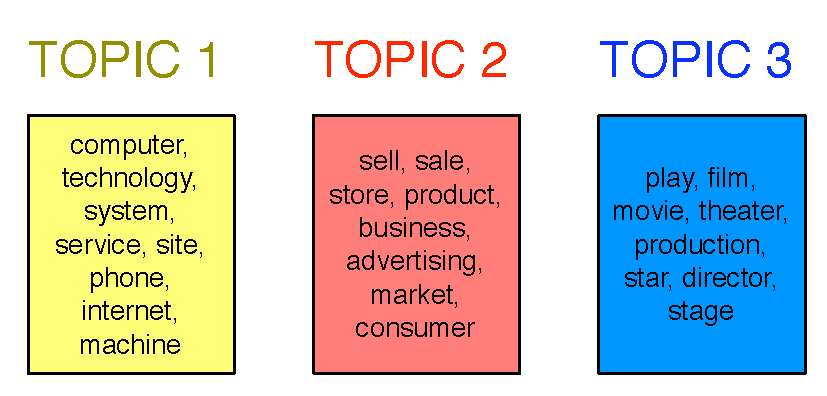
\includegraphics[width=0.9\linewidth]{reading_tea_leaves/figures/nyt_topics_wide}}
\end{center}
}

\frame{\frametitle{Conceptual Approach}

\begin{itemize}
\item For each document, what topics are expressed by that document?

\begin{center}
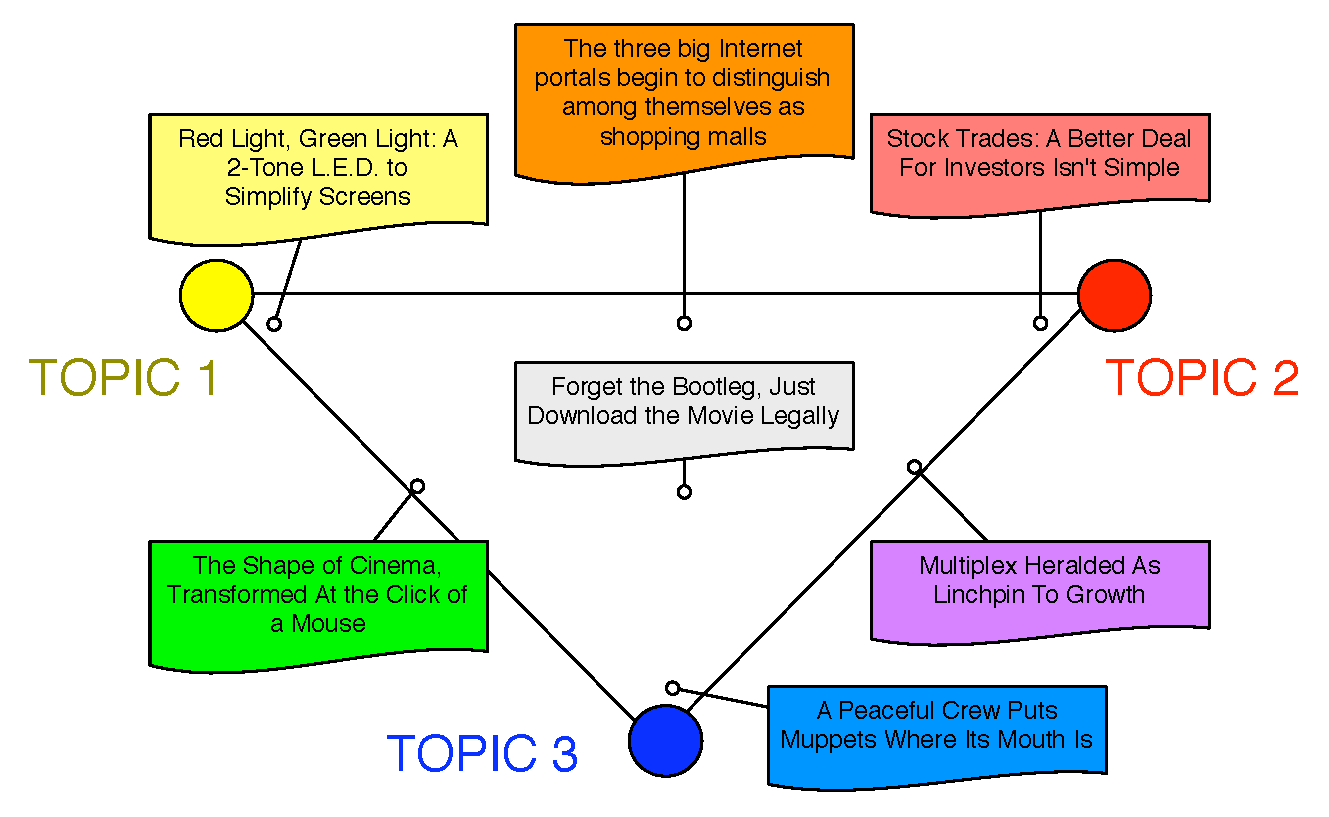
\includegraphics[width=0.9\linewidth]{topic_models/nyt_documents}
\end{center}

\end{itemize}
}

\iflong

\begin{frame}

\frametitle{Topics from \emph{Science}}

\begin{center}
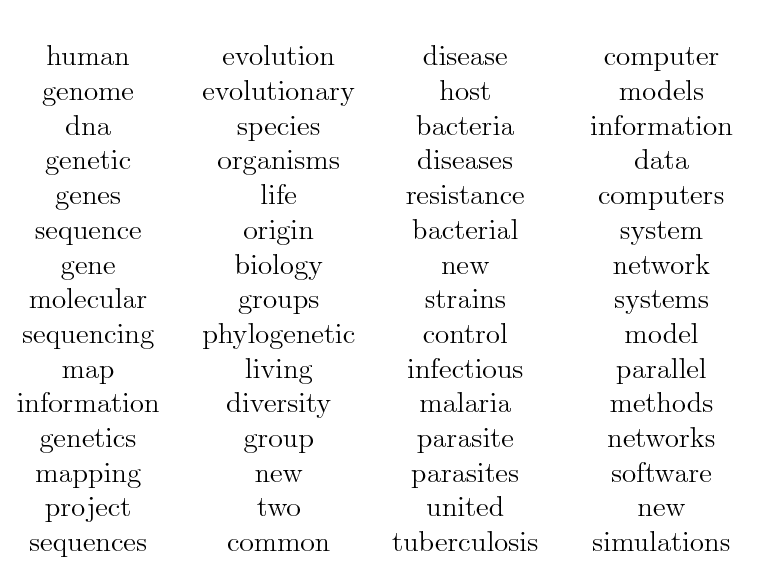
\includegraphics[width=0.8\linewidth]{topic_models/example_topics}
\end{center}

\end{frame}


\begin{frame}

\frametitle{Why should you care?}

\begin{itemize}
\item Neat way to explore / understand corpus collections
\begin{itemize}
	\item E-discovery
	\item Social media
	\item Scientific data
\end{itemize}
\item NLP Applications
\begin{itemize}
   \item POS Tagging~\cite{toutanova-08}
   \item Word Sense Disambiguation~\cite{boyd-graber-07}
   \item Word Sense Induction~\cite{brody-09}
   \item Discourse Segmentation~\cite{purver-06}
\end{itemize}
\item Psychology~\cite{griffiths-07}: word meaning, polysemy
\item Inference is (relatively) simple
\end{itemize}

\end{frame}

\frame
{
  \frametitle{Matrix Factorization Approach}

\begin{center}
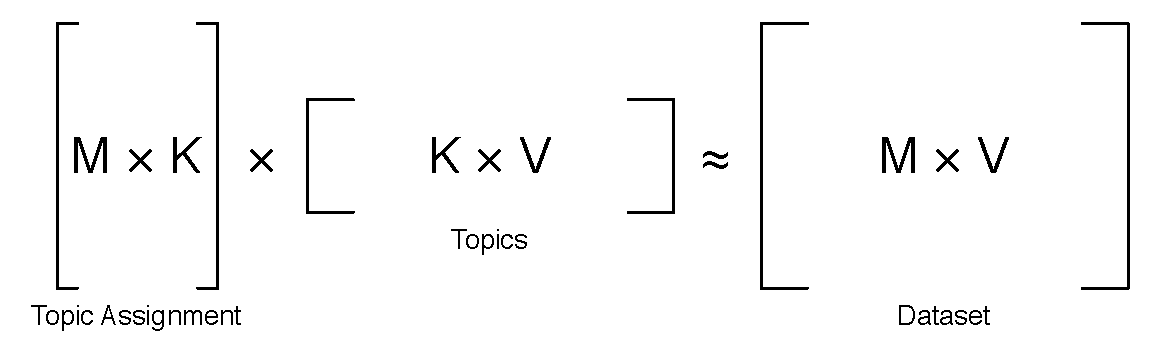
\includegraphics[width=0.9\linewidth]{topic_models/factorization.pdf}
\end{center}

\begin{columns}
\column{.5\textwidth}
\begin{block}{}
	\begin{itemize}
		\item[K] Number of topics
		\item[M] Number of documents
		\item[V] Size of vocabulary
	\end{itemize}
\end{block}
\column{.5\textwidth}
\pause
\begin{itemize}
\item If you use singular value decomposition (SVD), this technique is called latent semantic analysis.
\item Popular in information retrieval.
\end{itemize}
\end{columns}

}

\begin{frame}

\frametitle{Alternative: Generative Model}

\begin{itemize}
  \item How your data came to be
  \item Sequence of Probabilistic Steps
  \item Posterior Inference
\end{itemize}

\end{frame}

\begin{frame}
	\frametitle{Multinomial Distribution}

	\begin{itemize}
		\item Distribution over discrete outcomes
		\item Represented by non-negative vector that sums to one
		\item Picture representation
	\begin{center}
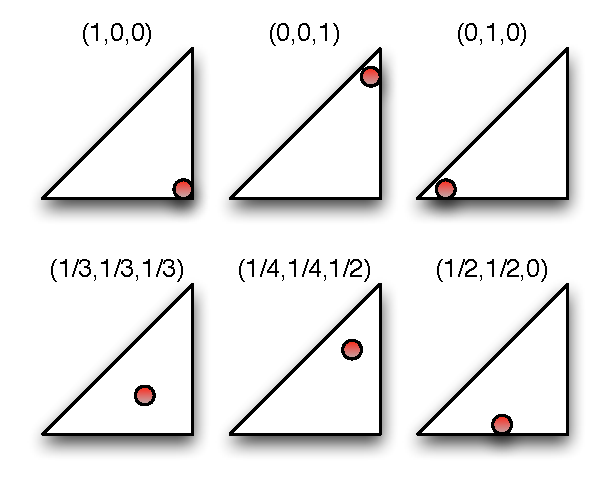
\includegraphics[width=0.4\linewidth]{topic_models/multinomial}
	\end{center}
		\pause
		\item Come from a Dirichlet distribution

	\end{itemize}


\end{frame}

\begin{frame}

\frametitle{Dirichlet Distribution}

\begin{center}
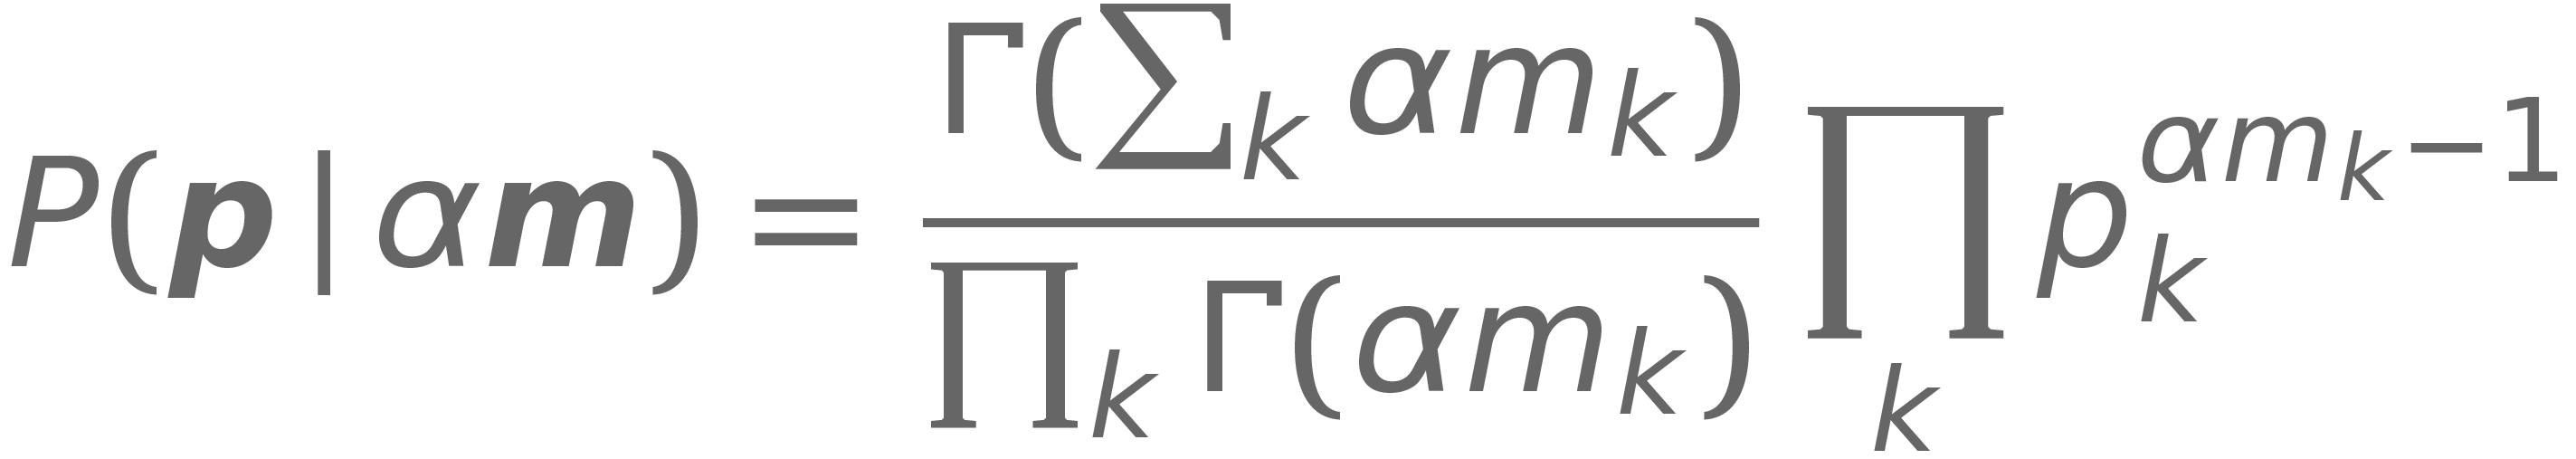
\includegraphics[width=0.4\linewidth]{topic_models/equations/dirichlet} \\ \bigskip
\pause
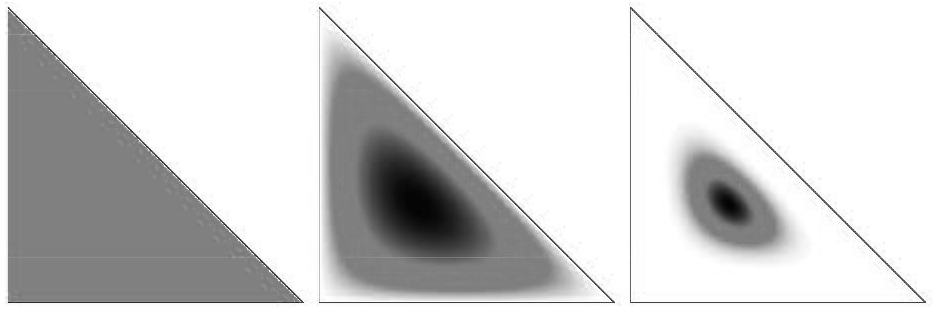
\includegraphics[width=0.6\linewidth]{topic_models/dirichlet_1} \\
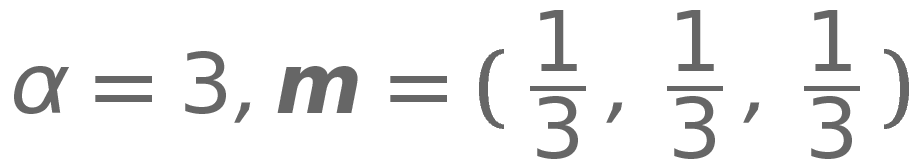
\includegraphics[width=0.2\linewidth]{topic_models/equations/dirichlet_params_1} 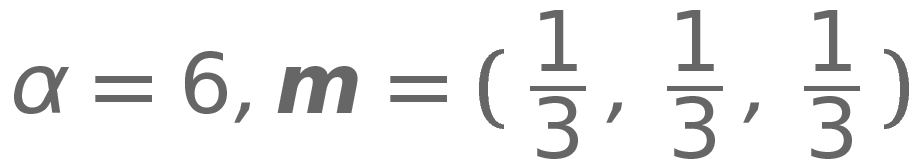
\includegraphics[width=0.2\linewidth]{topic_models/equations/dirichlet_params_2} 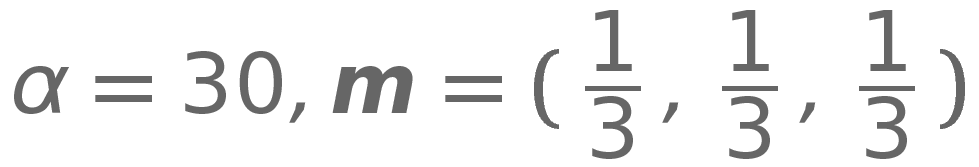
\includegraphics[width=0.2\linewidth]{topic_models/equations/dirichlet_params_3} \\
\pause

\includegraphics[width=0.6\linewidth]{topic_models/dirichlet_2} \\
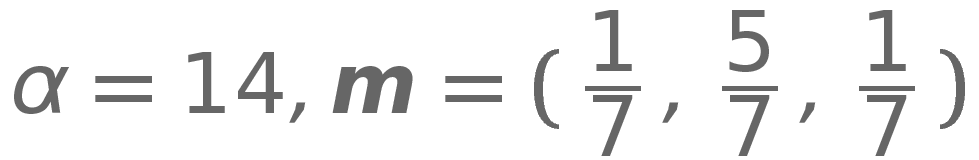
\includegraphics[width=0.2\linewidth]{topic_models/equations/dirichlet_params_4} 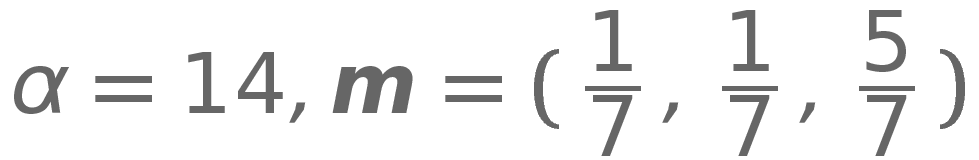
\includegraphics[width=0.2\linewidth]{topic_models/equations/dirichlet_params_5} 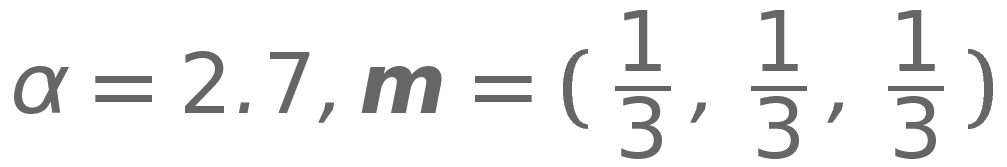
\includegraphics[width=0.2\linewidth]{topic_models/equations/dirichlet_params_6} \\
\end{center}

\end{frame}

\begin{frame}
\frametitle{Dirichlet Distribution}
\begin{center}
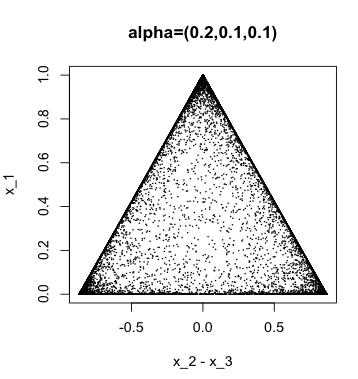
\includegraphics[width=0.5\linewidth]{topic_models/sparsity}
\end{center}
\end{frame}

\fi
\ifconjugacy

\begin{frame}
\frametitle{Dirichlet Distribution}
\begin{itemize}
  \item If ${\bm \phi} \sim \Dir(\alpha)$, ${\bm w} \sim \Mult(\phi)$, and $n_k = |\{ w_i : w_i = k\}|$ then
  \begin{align}
  	p(\phi | \alpha, {\bm w}) & \propto p({\bm w} | \phi) p(\phi | \alpha) \\
	                       & \propto  \prod_{k} \phi^{n_k} \pause  \prod_k { \phi^{\alpha_k - 1}} \\
	                       & \propto \prod_k \phi^{\alpha_k + n_k - 1}
  \end{align}
  \item Conjugacy: this {\bf posterior} has the same form as the {\bf prior}
\end{itemize}
\end{frame}

\fi

\ifhighlevel

\else

\frame
{
  \frametitle{Generative Model Approach}

\begin{center}
\only<1>{ 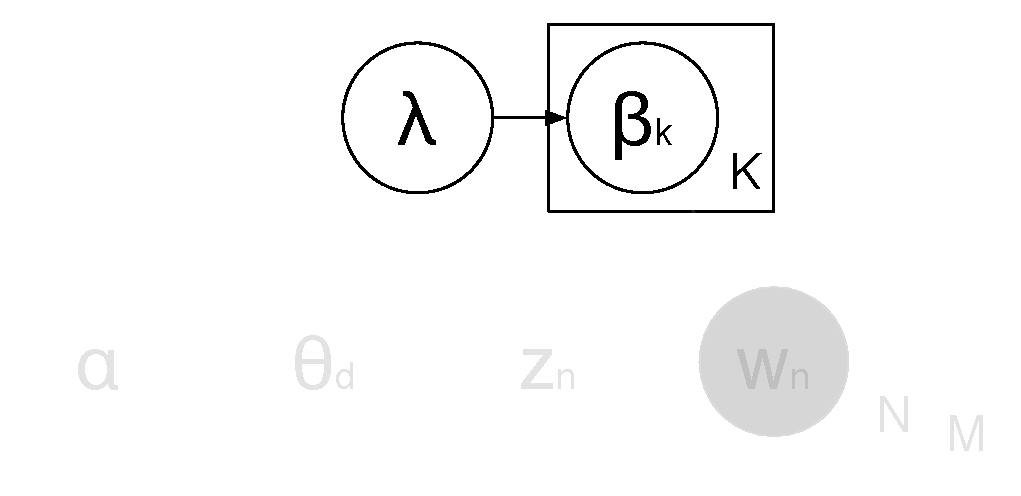
\includegraphics[scale=0.4]{topic_models/lda1.pdf} }
\only<2>{ 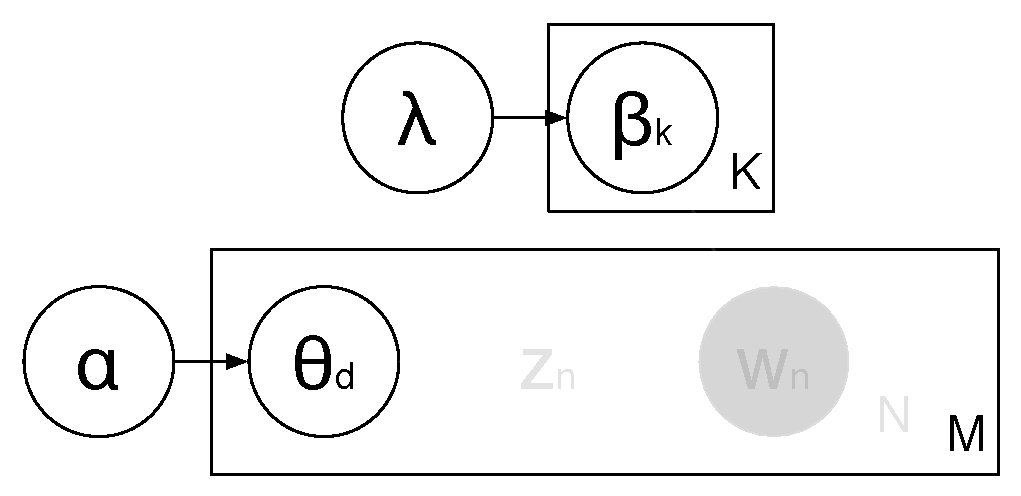
\includegraphics[scale=0.4]{topic_models/lda2.pdf} }
\only<3>{ 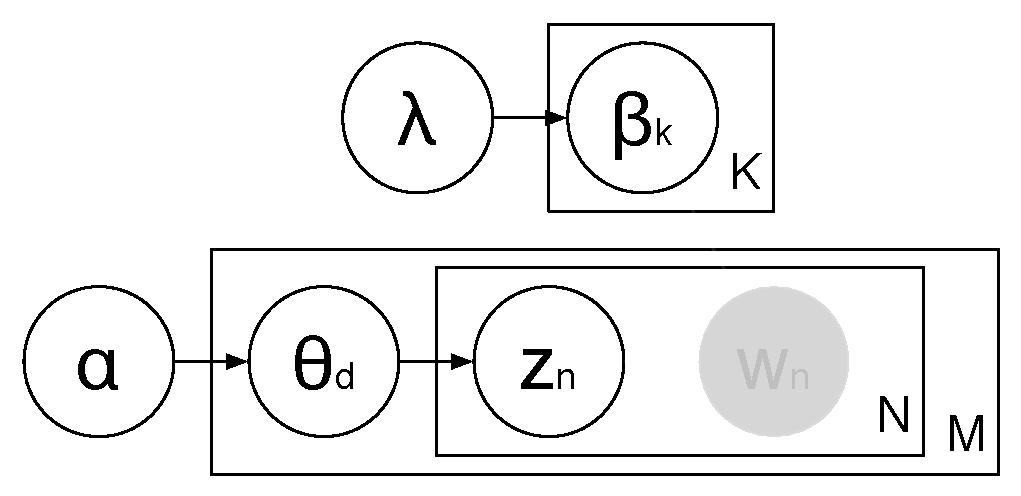
\includegraphics[scale=0.4]{topic_models/lda3.pdf} }
\only<4->{ 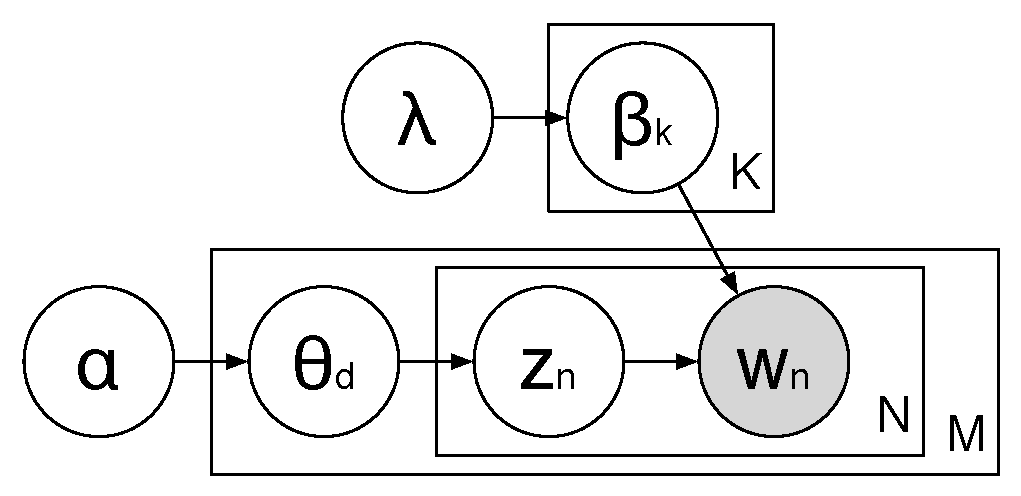
\includegraphics[scale=0.4]{topic_models/lda4.pdf} }
\end{center}

\begin{itemize}
\item<1-> For each topic $k \in \{1, \dots, K\}$, draw a multinomial distribution $\beta_k$ from a Dirichlet distribution with parameter $\lambda$
\item<2-> For each document $d \in \{1, \dots, M\}$, draw a multinomial distribution $\theta_d$ from a Dirichlet distribution with parameter $\alpha$
\item<3-> For each word position $n \in \{1, \dots, N\}$, select a hidden topic $z_n$ from the multinomial distribution parameterized by $\theta$.
\item<4-> Choose the observed word $w_n$ from the distribution $\beta_{z_n}$.
\end{itemize}

\only<5->{We use statistical inference to uncover the most likely unobserved variables given observed data.}
}

\fi

\begin{frame}
\frametitle{Topic Models: What's Important}
\begin{itemize}
\item Topic models \only<2>{(latent variables)}
\begin{itemize}
\ifhighlevel
	\item Topics to words
	\item Documents to topics
\else
	\item Topics to words---multinomial distribution
	\item Documents to topics---multinomial distribution
\fi
\end{itemize}
\item Focus in this talk: statistical methods
  \begin{itemize}
    \item Model: story of how your data came to be
    \item Latent variables: missing pieces of your story
    \item Statistical inference: filling in those missing pieces
  \end{itemize}
\item We use latent Dirichlet allocation (LDA)~\cite{blei-03}, a fully Bayesian
  version of pLSI~\cite{hofmann-99}, probabilistic version of
  LSA~\cite{landauer-97}
\end{itemize}

\end{frame}

\ifevaluation


\frame{
\frametitle{Evaluation}
\begin{center}
%\only<1>{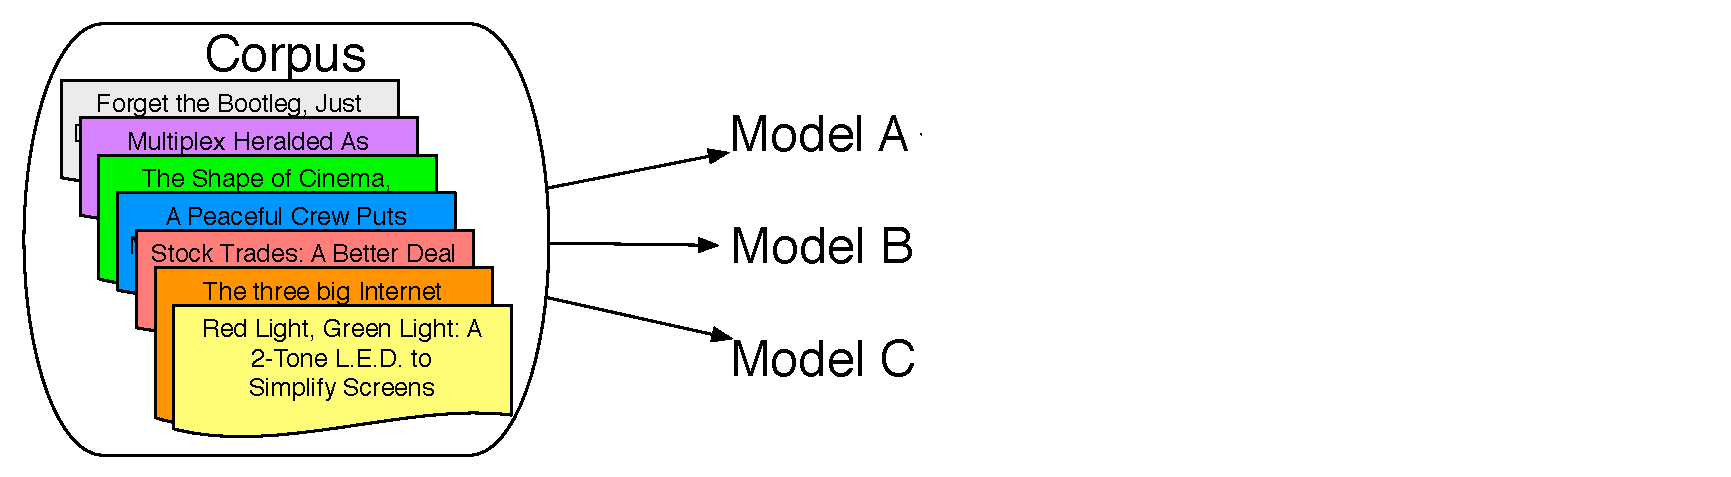
\includegraphics[width=0.9\linewidth]{reading_tea_leaves/figures/heldout_1} }
\only<1>{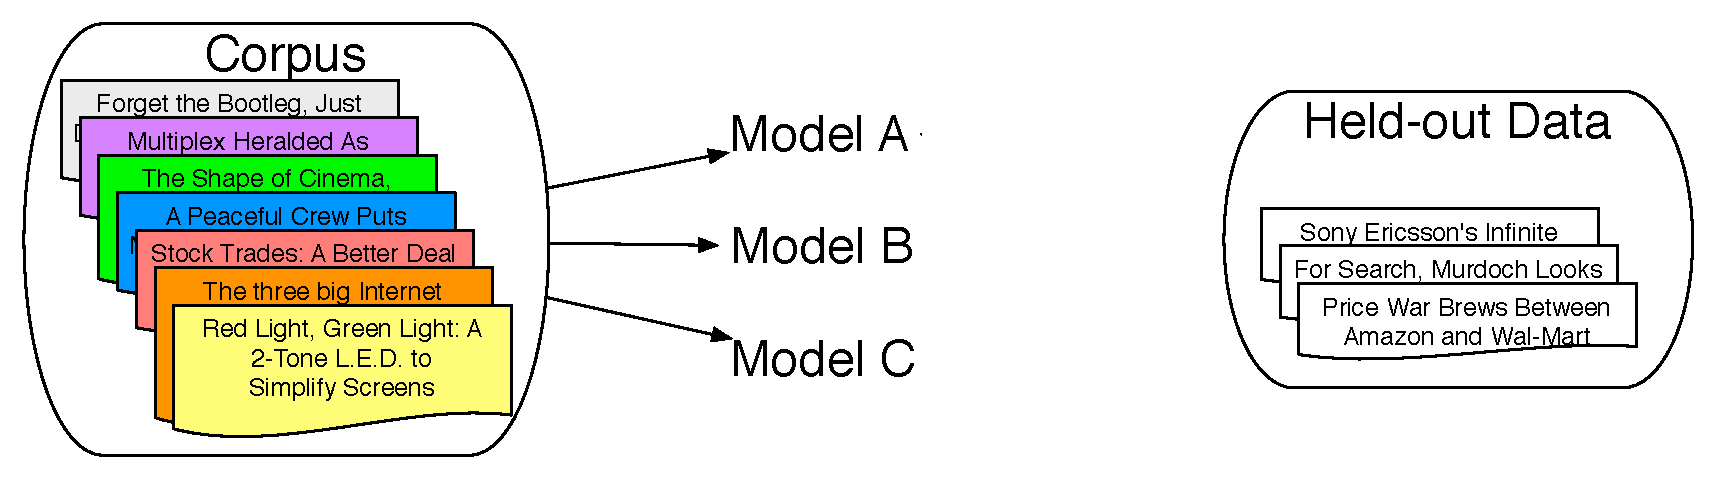
\includegraphics[width=\linewidth]{reading_tea_leaves/figures/heldout_2} }
%\only<3>{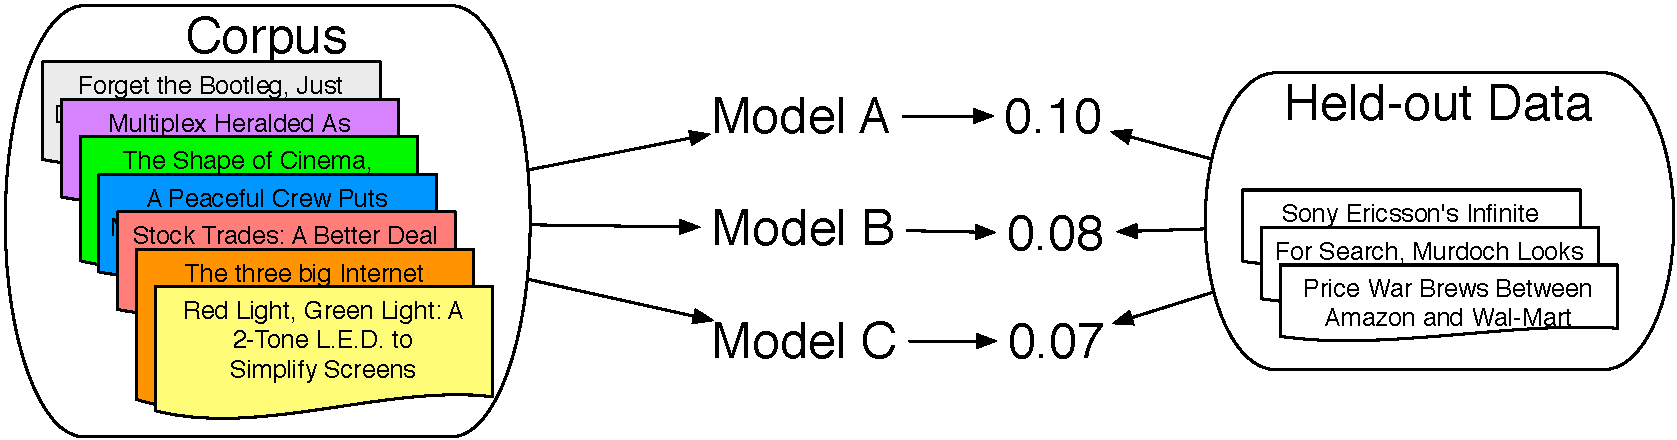
\includegraphics[width=\linewidth]{reading_tea_leaves/figures/heldout_3} }
\only<2>{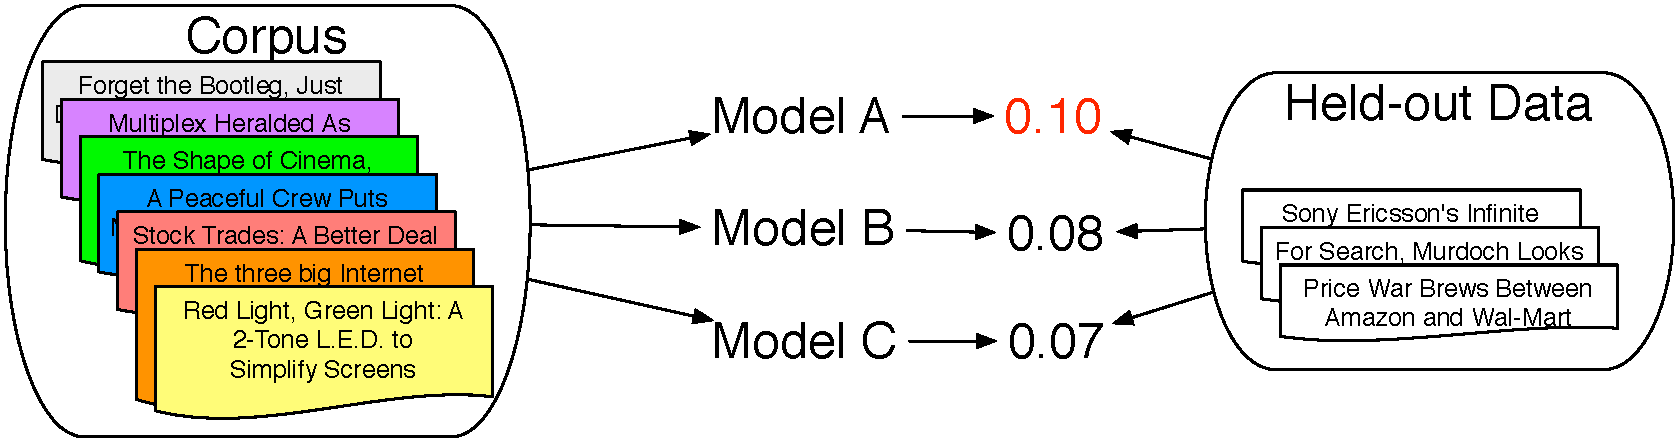
\includegraphics[width=\linewidth]{reading_tea_leaves/figures/heldout_4}  \\
	\large Measures predictive power, not what the topics are}
\end{center}

\begin{center}
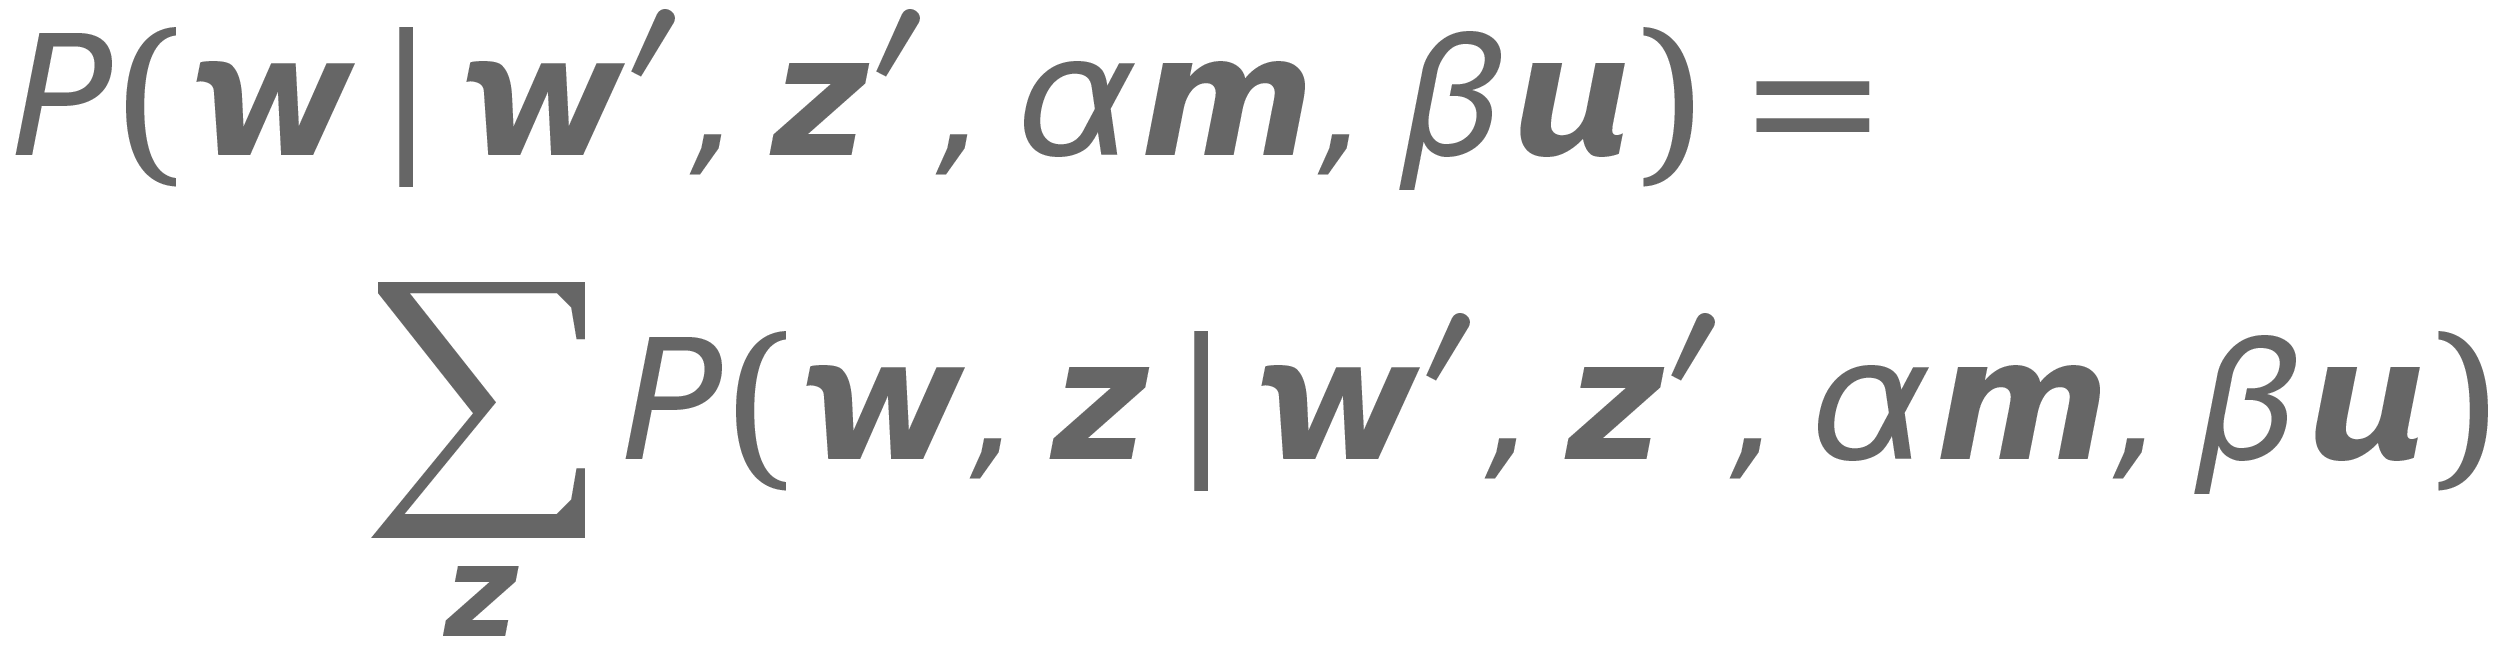
\includegraphics[width=0.5\linewidth]{topic_models/equations/evaluation} \\
How you compute it is important too~\cite{wallach-09b}
\end{center}

}

\frame{
  \frametitle{Word Intrusion}

  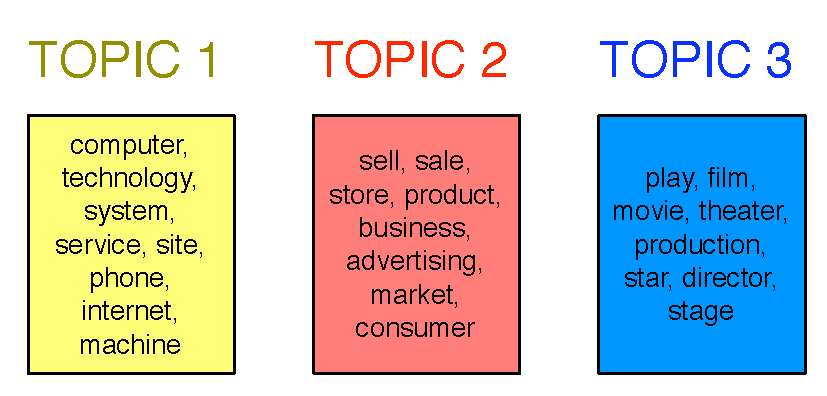
\includegraphics[width=\linewidth]{reading_tea_leaves/figures/nyt_topics_wide}
}


\frame{
  \frametitle{Word Intrusion}

  \begin{enumerate}
    \item Take the highest probability words from a topic

      \begin{block}{Original Topic}
        dog, cat, horse, pig, cow
      \end{block}
\pause
    \item Take a high-probability word from another topic and add it
      \begin{block}{Topic with Intruder}
        dog, cat, \alert<2->{apple}, horse, pig, cow
      \end{block}
\pause
     \item We ask users to find the word that doesn't belong
  \end{enumerate}
\begin{block}{Hypothesis}
If the topics are interpretable, users will consistently choose true intruder
\end{block}
}

\frame{
\frametitle{Word Intrusion}
\begin{center}
\only<1>{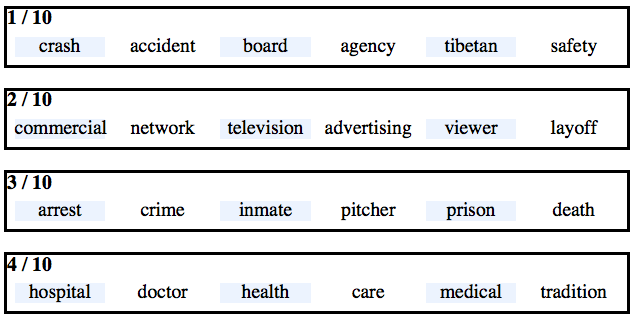
\includegraphics[width=\linewidth]{reading_tea_leaves/tasks/word1}  }
\only<2>{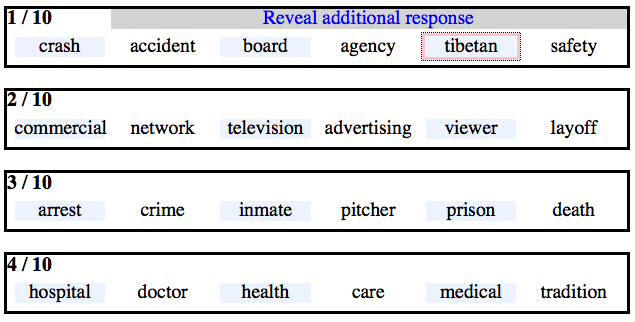
\includegraphics[width=\linewidth]{reading_tea_leaves/tasks/word2}  }
\pause
  \begin{itemize}
    \item Order of words was shuffled
    \item Which intruder was selected varied
    \item Model precision: percentage of users who clicked on intruder
  \end{itemize}

\end{center}
}

\frame{
\frametitle{Word Intrusion: Which Topics are Interpretable?}
  \begin{block}{New York Times, 50 LDA Topics}
    \begin{center}
      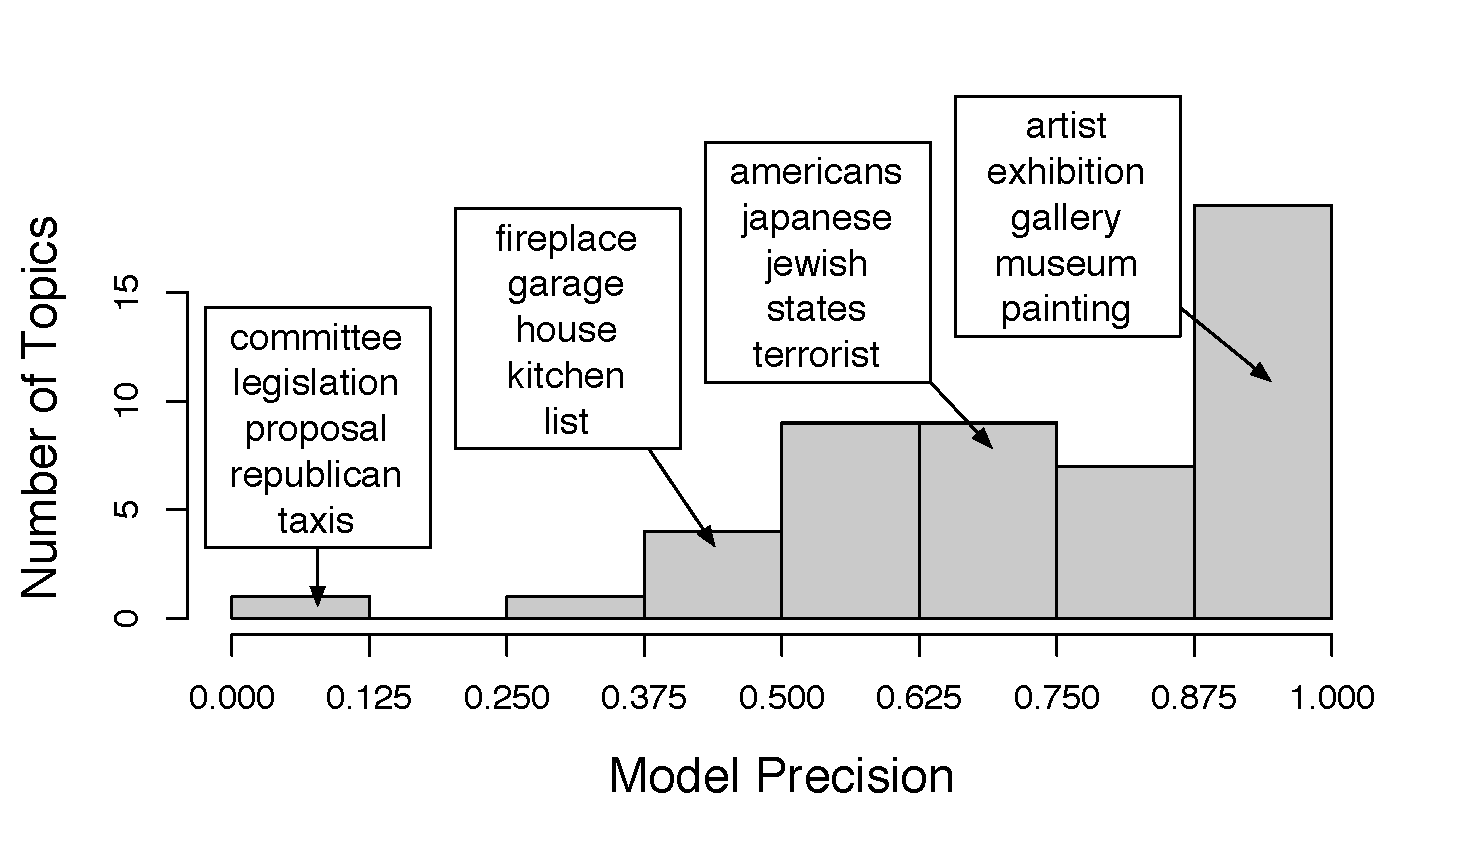
\includegraphics[width=0.8\linewidth]{reading_tea_leaves/figures/topic_precision}
    \end{center}
  \end{block}
  \begin{center}
    Model Precision: percentage of correct intruders found
  \end{center}
}



\frame{

\frametitle{Interpretability and Likelihood}
\begin{center}
\only<1>{Model Precision on New York Times}
\only<2>{Topic Log Odds on Wikipedia}
\end{center}

\begin{columns}
\column{.85\linewidth}
\begin{flushright}
  \only<1>{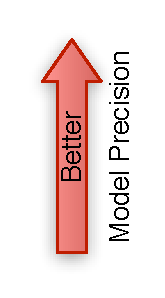
\includegraphics[scale=\graphscale]{reading_tea_leaves/tasks/mp}}
  \only<2>{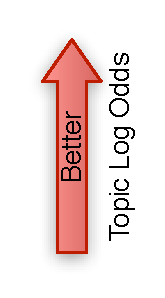
\includegraphics[scale=\graphscale]{reading_tea_leaves/tasks/tlo}}
  \only<1>{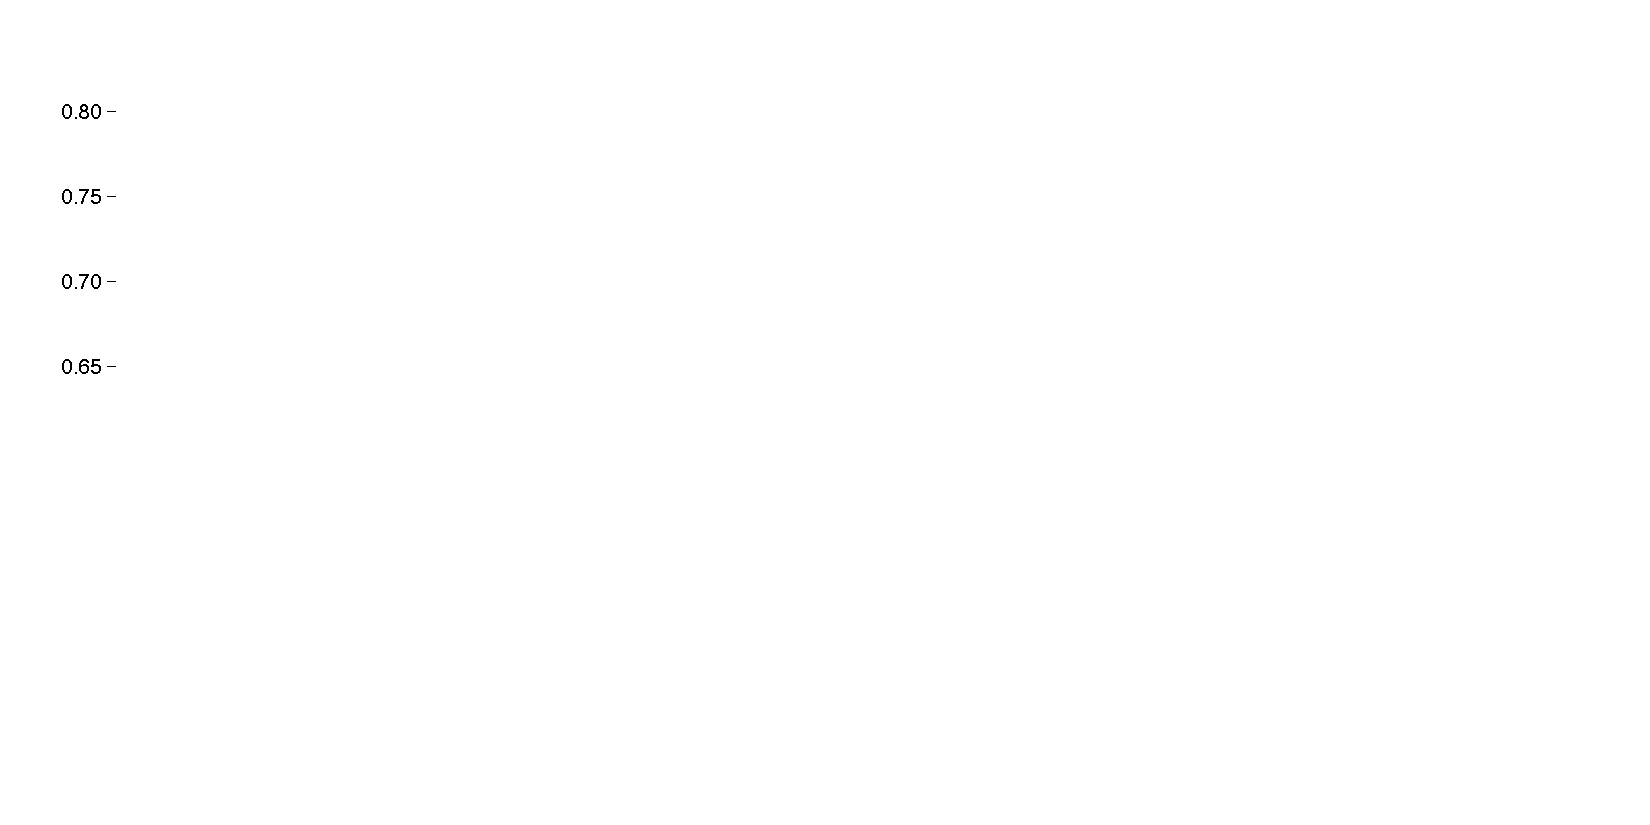
\includegraphics[scale=\graphscale]{reading_tea_leaves/tasks/mp_y}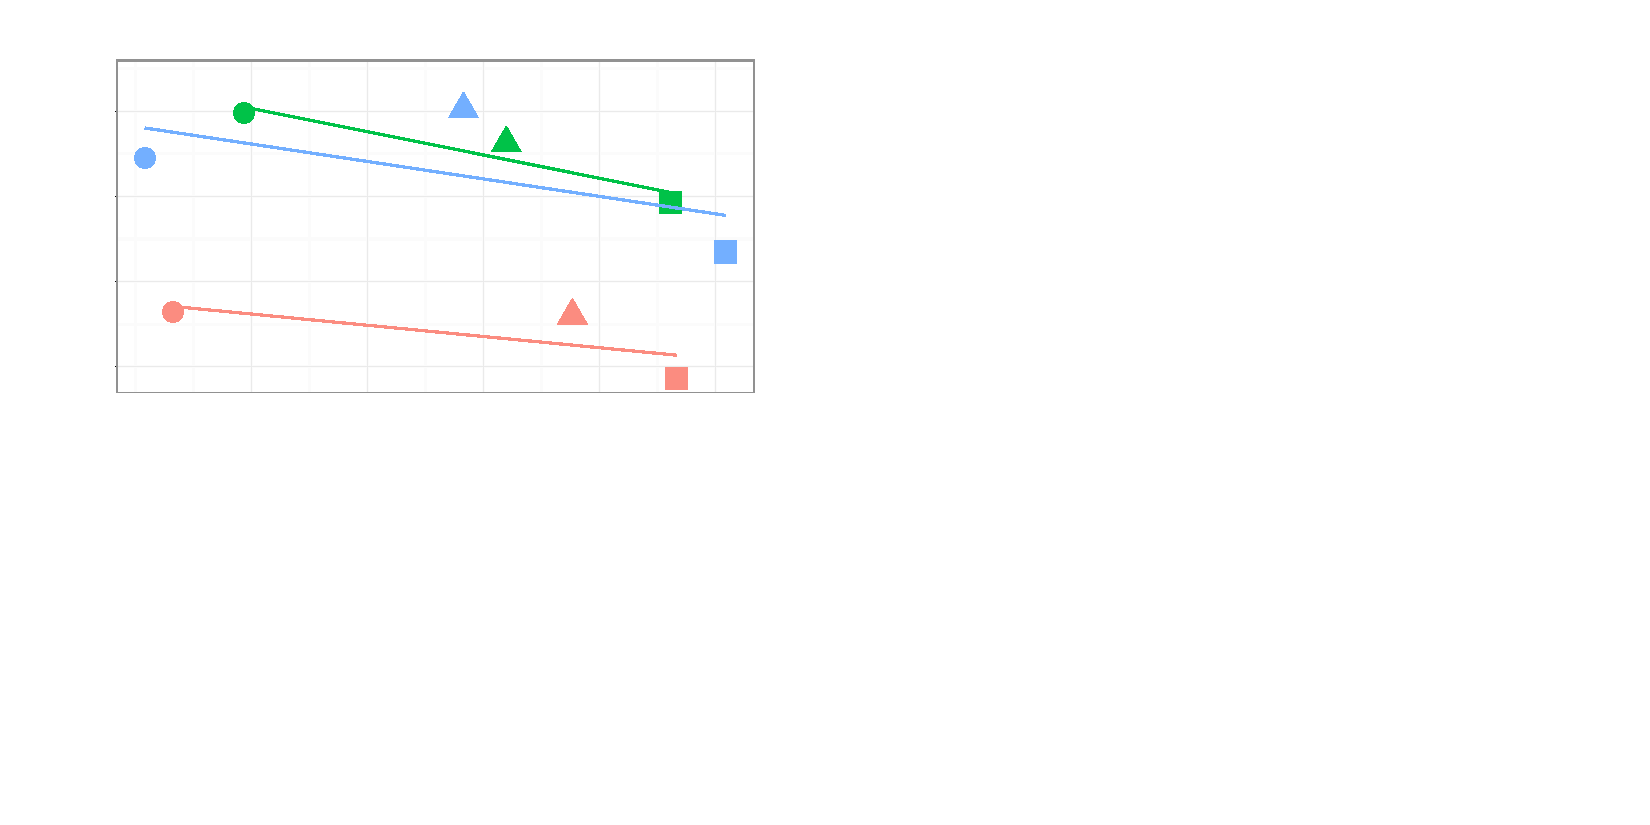
\includegraphics[scale=\graphscale]{reading_tea_leaves/tasks/nyt_mp}}
  \only<2>{
\includegraphics[scale=\graphscale]{reading_tea_leaves/tasks/tlo_y}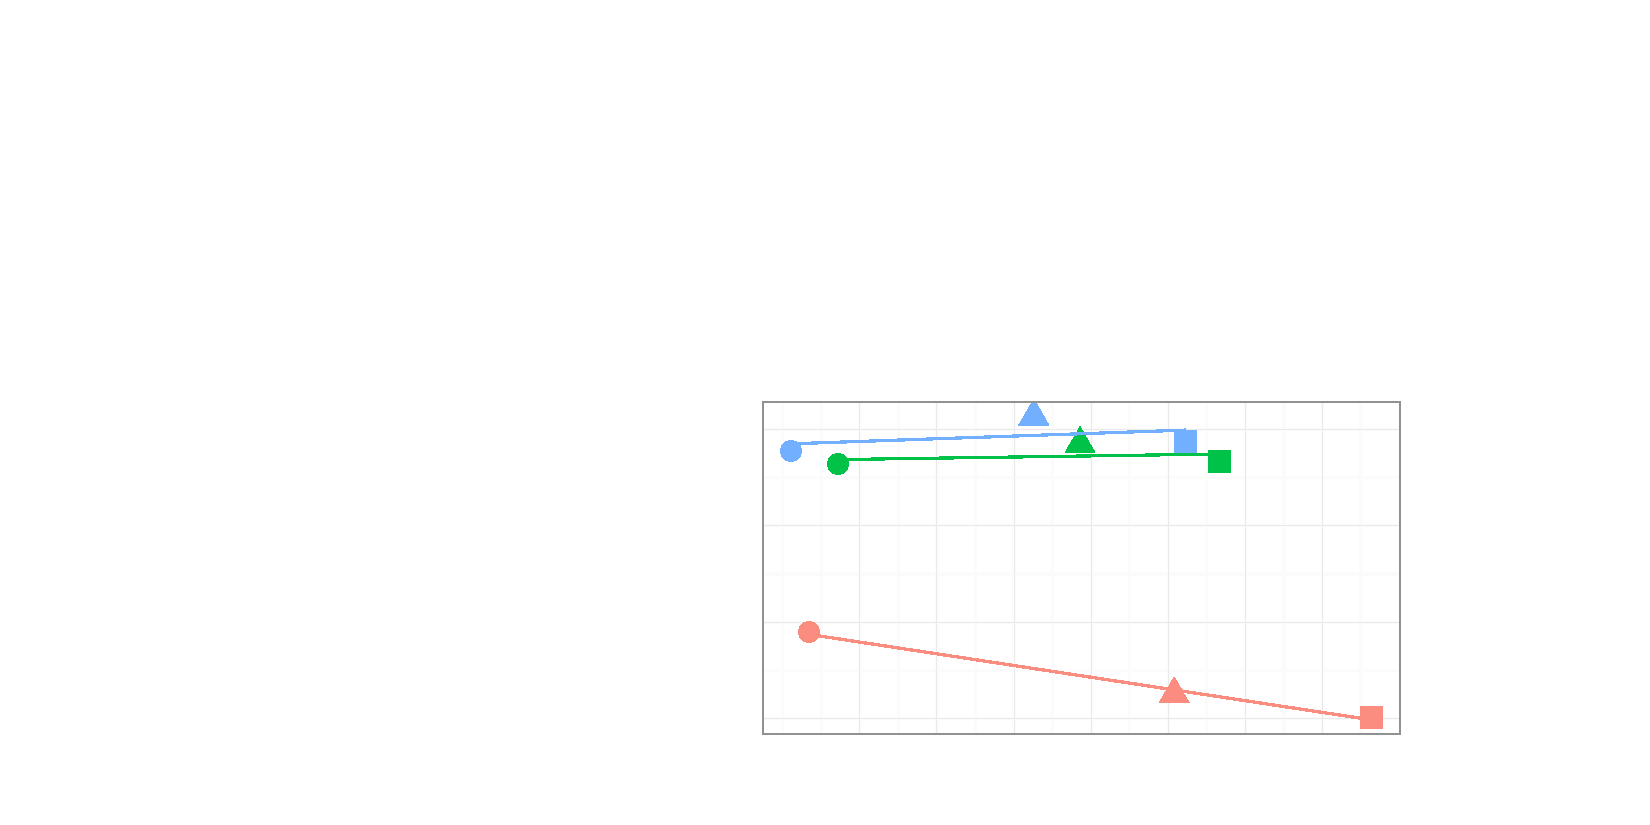
\includegraphics[scale=\graphscale]{reading_tea_leaves/tasks/wiki_tlo}} \\
  \only<1>{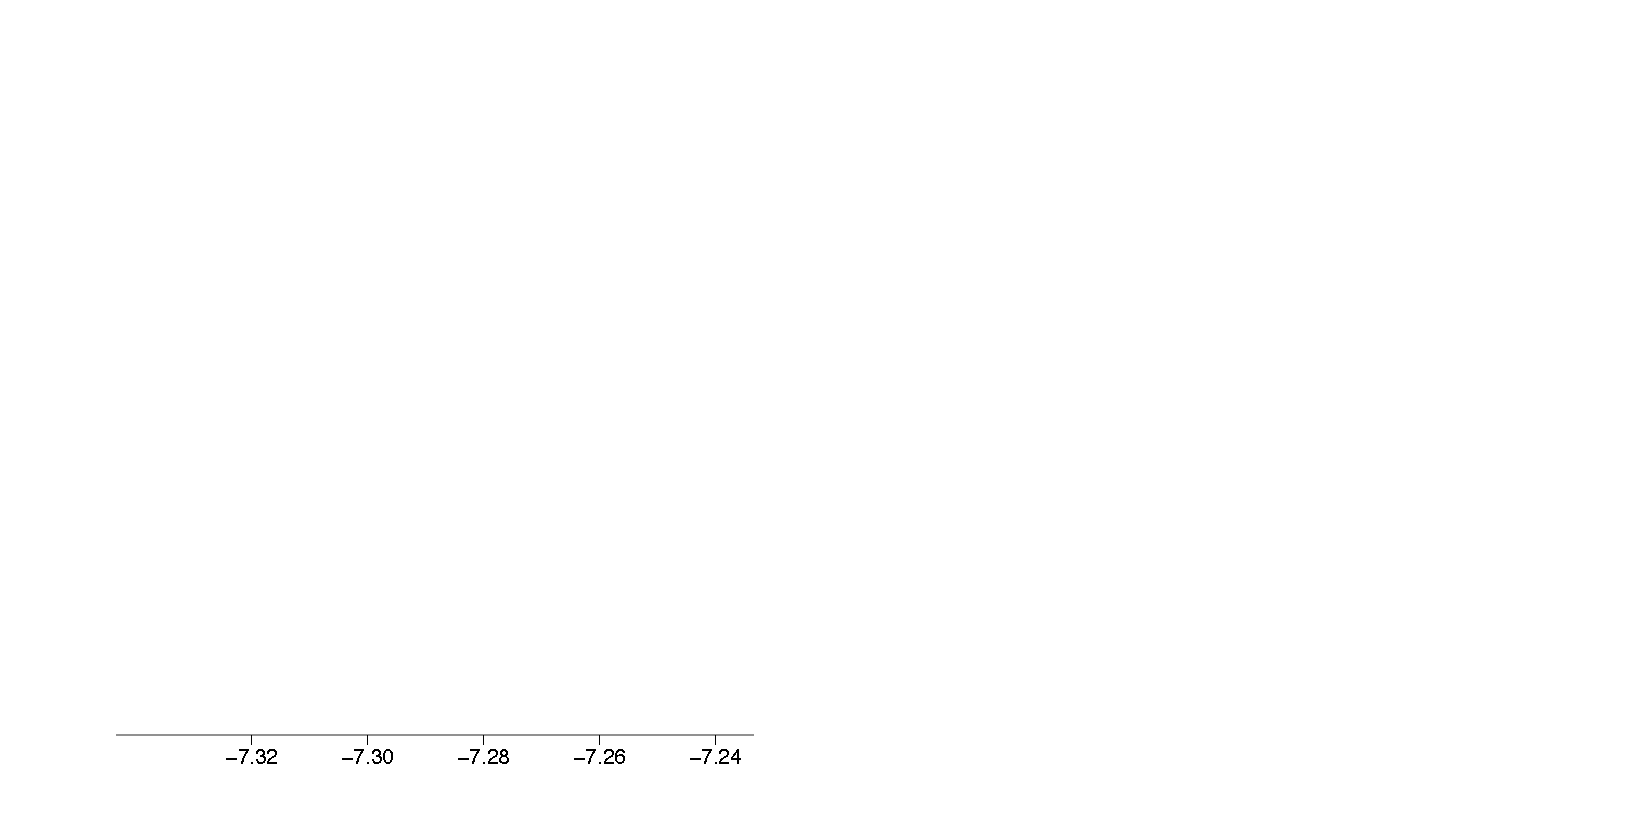
\includegraphics[scale=\graphscale]{reading_tea_leaves/tasks/nyt_x}}
  \only<2>{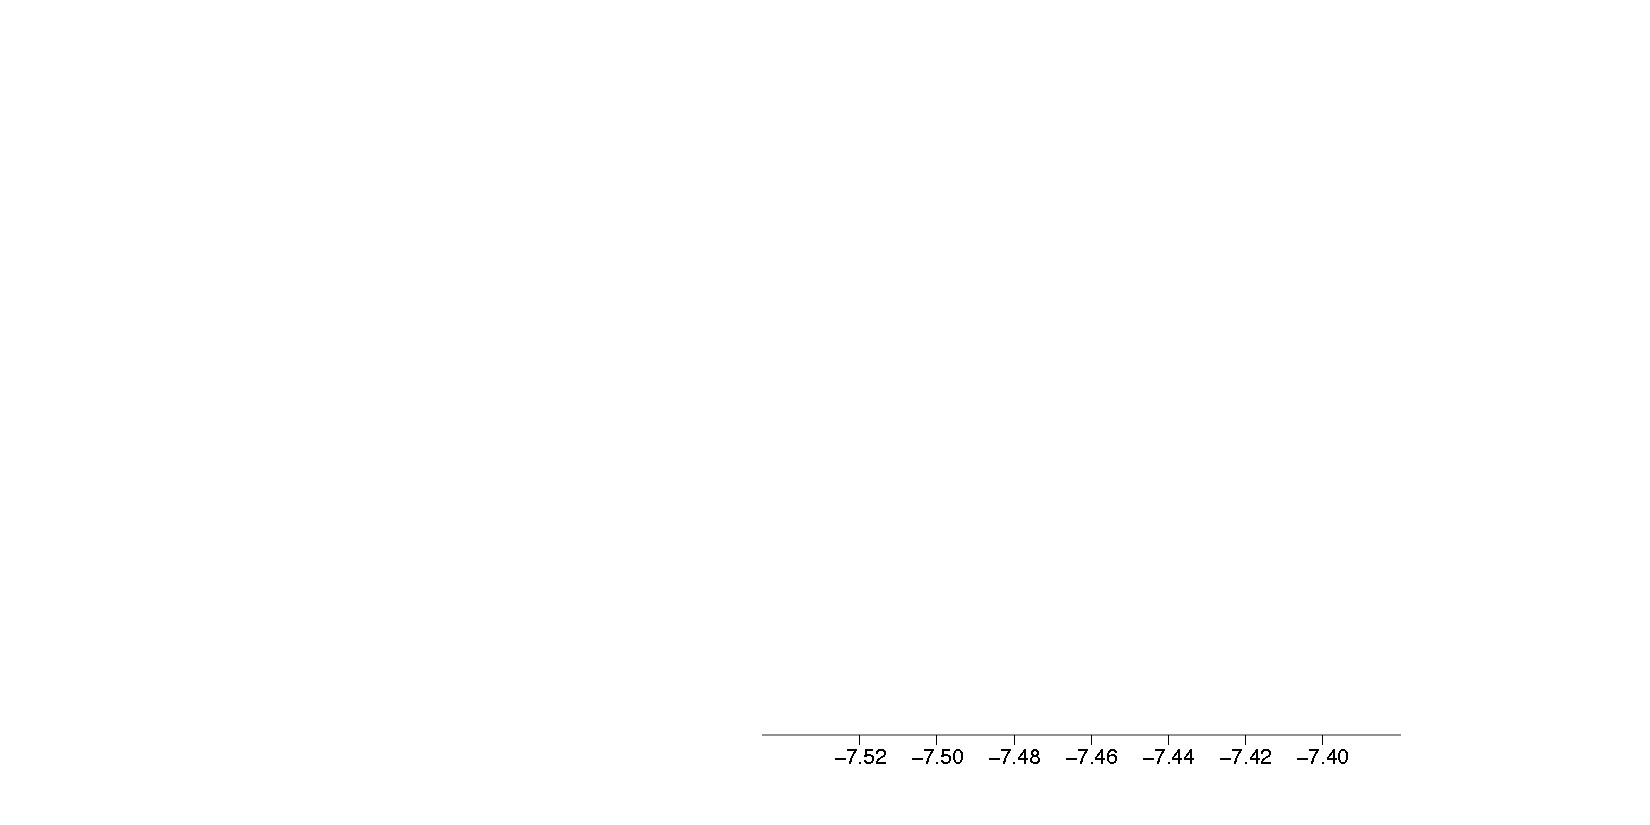
\includegraphics[scale=\graphscale]{reading_tea_leaves/tasks/wiki_x}}
\end{flushright}
\column{.15\linewidth}
  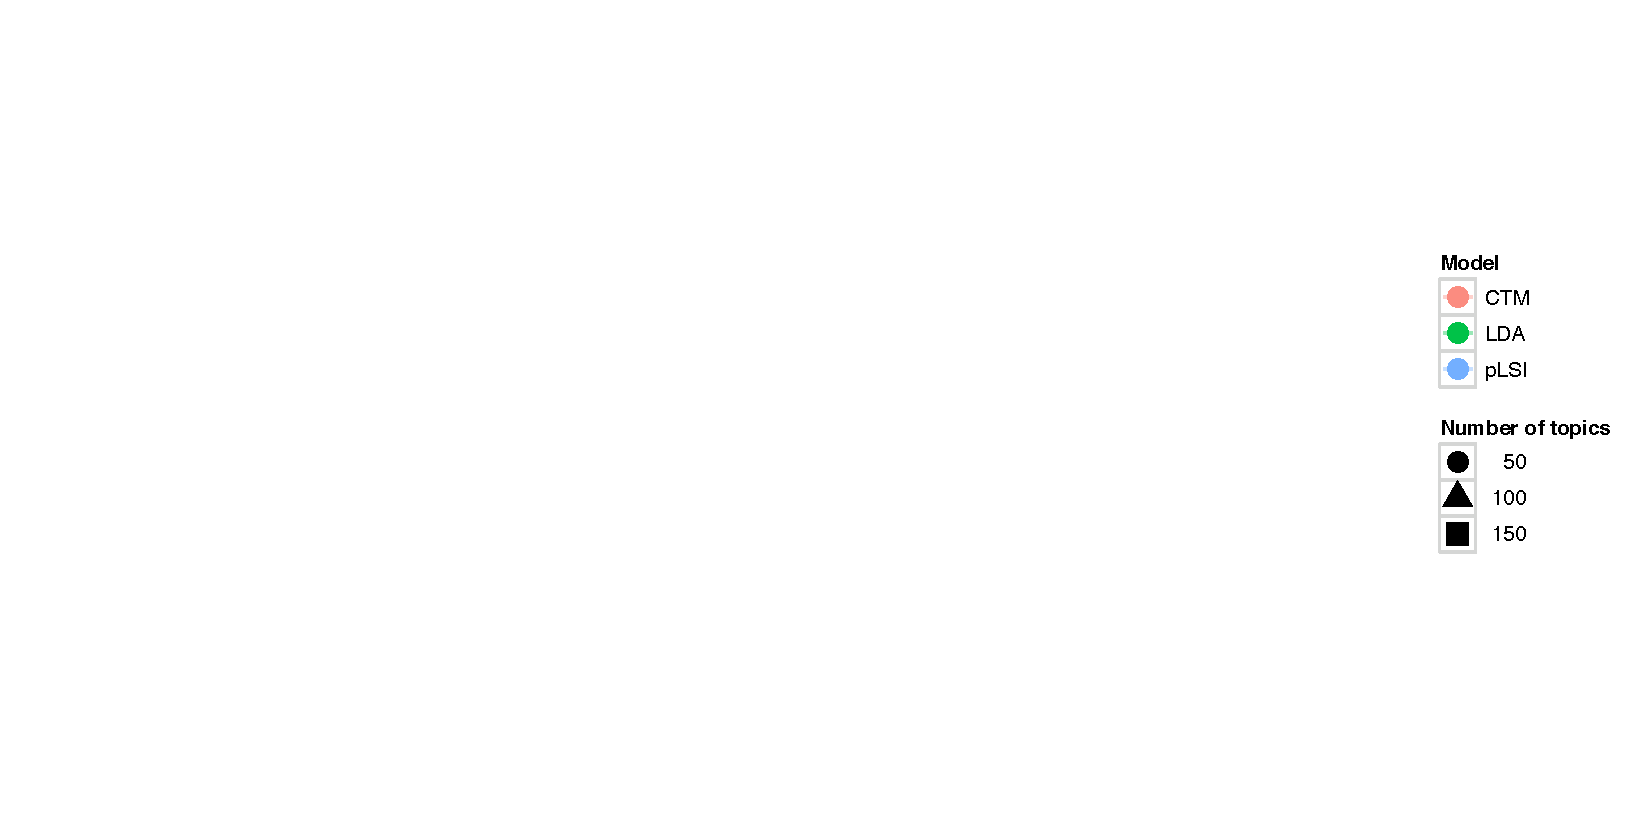
\includegraphics[scale=\graphscale]{reading_tea_leaves/tasks/legend}
\end{columns}
\vspace{-0.75cm}
\begin{center}
  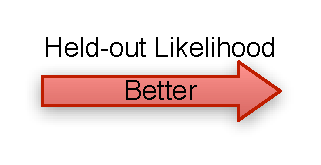
\includegraphics[scale=\graphscale]{reading_tea_leaves/tasks/held-out} \\
\only<1> {within a model, higher likelihood $\not =$ higher interpretability}
\only<2> {across models, higher likelihood $\not =$ higher interpretability}
\end{center}
}


\begin{frame}
  \frametitle{Evaluation Takeaway}

  \begin{itemize}
    \item Measure what you care about~\cite{chang-09c}
      \item If you care about prediction, likelihood is good
\item If you care about a particular task, measure that
    \end{itemize}

\end{frame}

\fi



\fi

\ifhighlevel

\else

\frame{
	\frametitle{Foundation: sLDA}

	\begin{columns}
		\column{.5\linewidth}
		   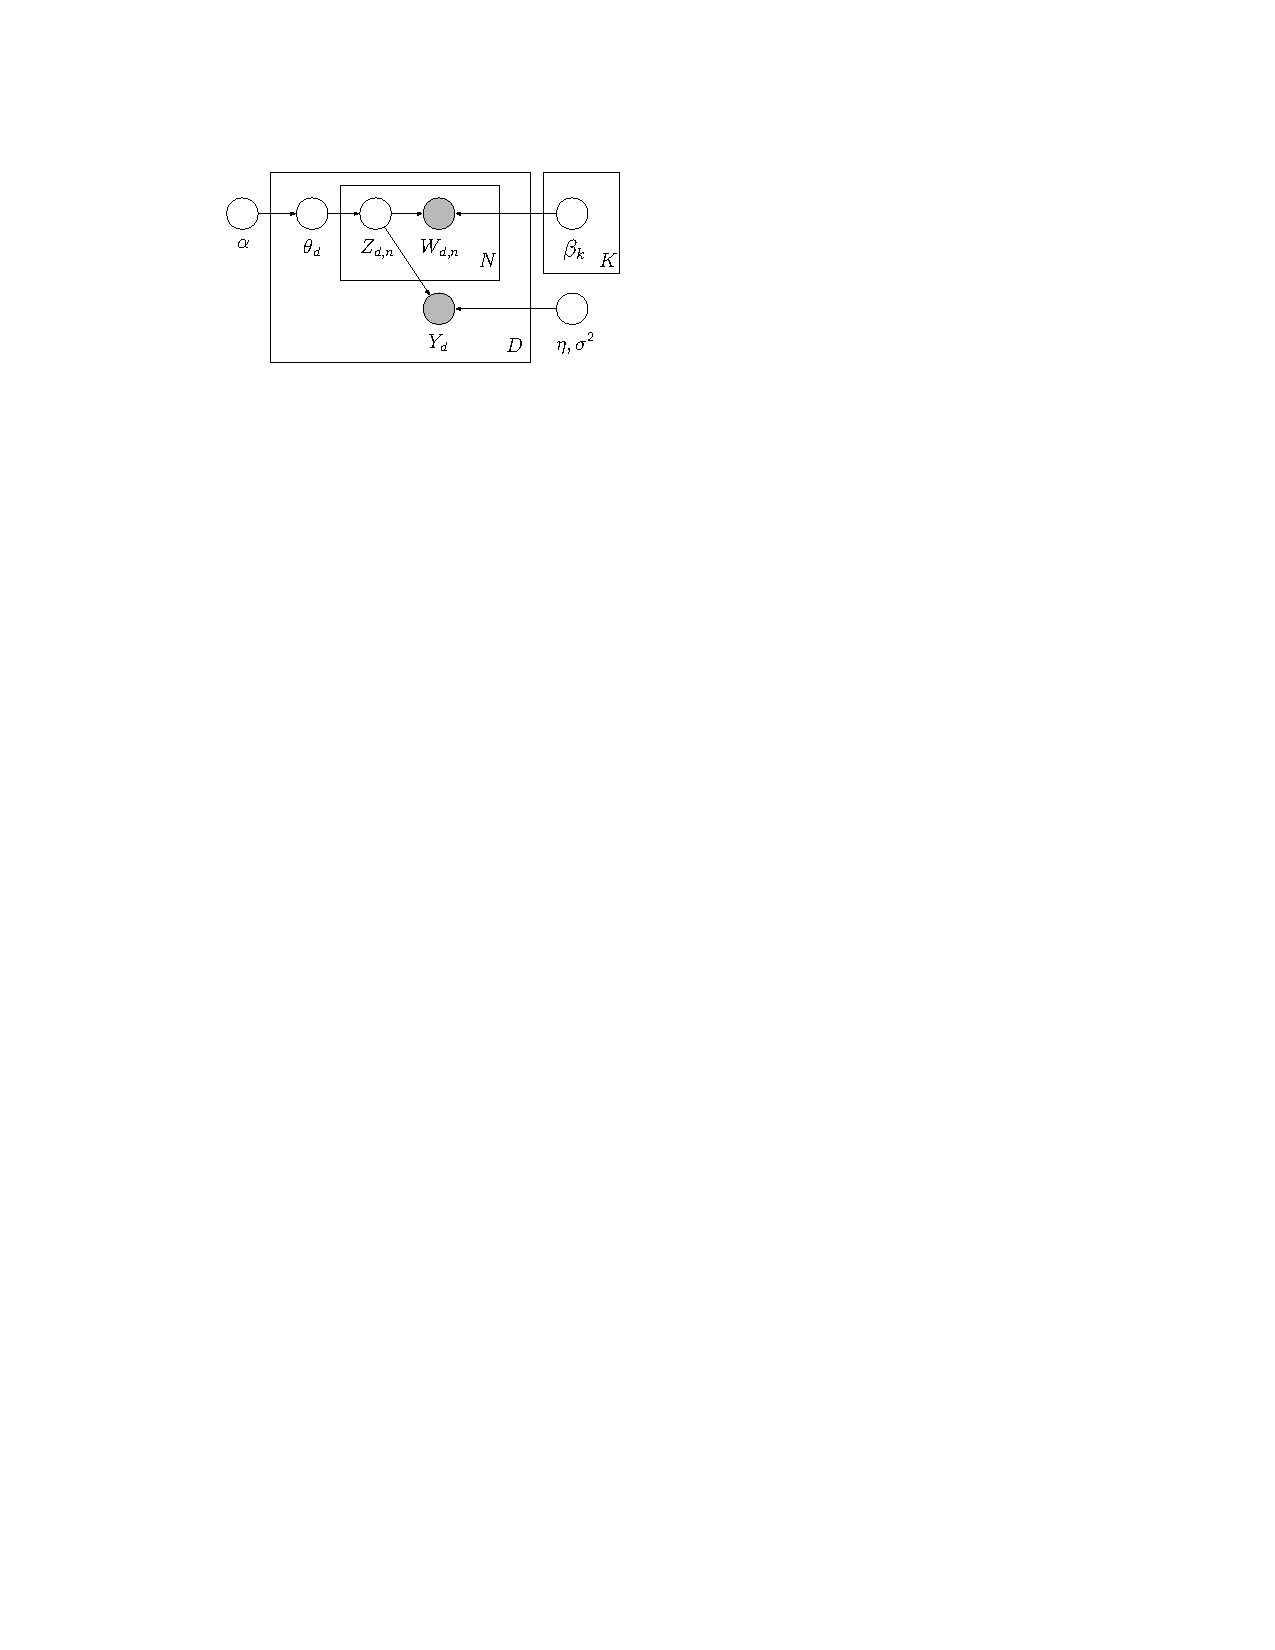
\includegraphics[width=1\linewidth]{mlslda/slda}
			\begin{center}
			supervised latent Dirichlet allocation \cite{blei-07b}
			\end{center}
		\column{.5\linewidth}
		  \begin{block}{Generative Process}
	\begin{enumerate}
		\item For document $d = 1 \dots D$:
		\begin{enumerate}
			\item Draw distribution over topics $\theta_d \sim \mbox{Dir}(\alpha)$
			\item For each word $n = 1 \dots d_n$
				\begin{enumerate}
					\item Draw a topic list assignment	$z_{d,n} \sim \mbox{Discrete}(\theta_d)$
					\item Draw word $w_{d,n}$ from topic list distribution $w_{d,n} \sim \mbox{Discrete}(\beta_{z_{d,n}})$
				\end{enumerate}
			\item Draw response $y_d \sim \mbox{Norm}(\eta^{\top} \bar{z}, \sigma^2)$
		\end{enumerate}
	\end{enumerate}


		  \end{block}
	\end{columns}

	\begin{center}
Topic lists $\beta$, topic assignments $z$, regression parameters $\eta$ learned via posterior inference
	\end{center}
}

\fi

\begin{frame}{Foundation: SLDA}

  Supervised Latent Dirichlet Allocation~\cite{blei-07b}

	\begin{block}{Scoring a Document}
		\begin{itemize}
			\item Each topic has a score
			\item Each word has a topic
			\item Document score is the average of all word scores
		\end{itemize}
	\end{block}

	\begin{center}
	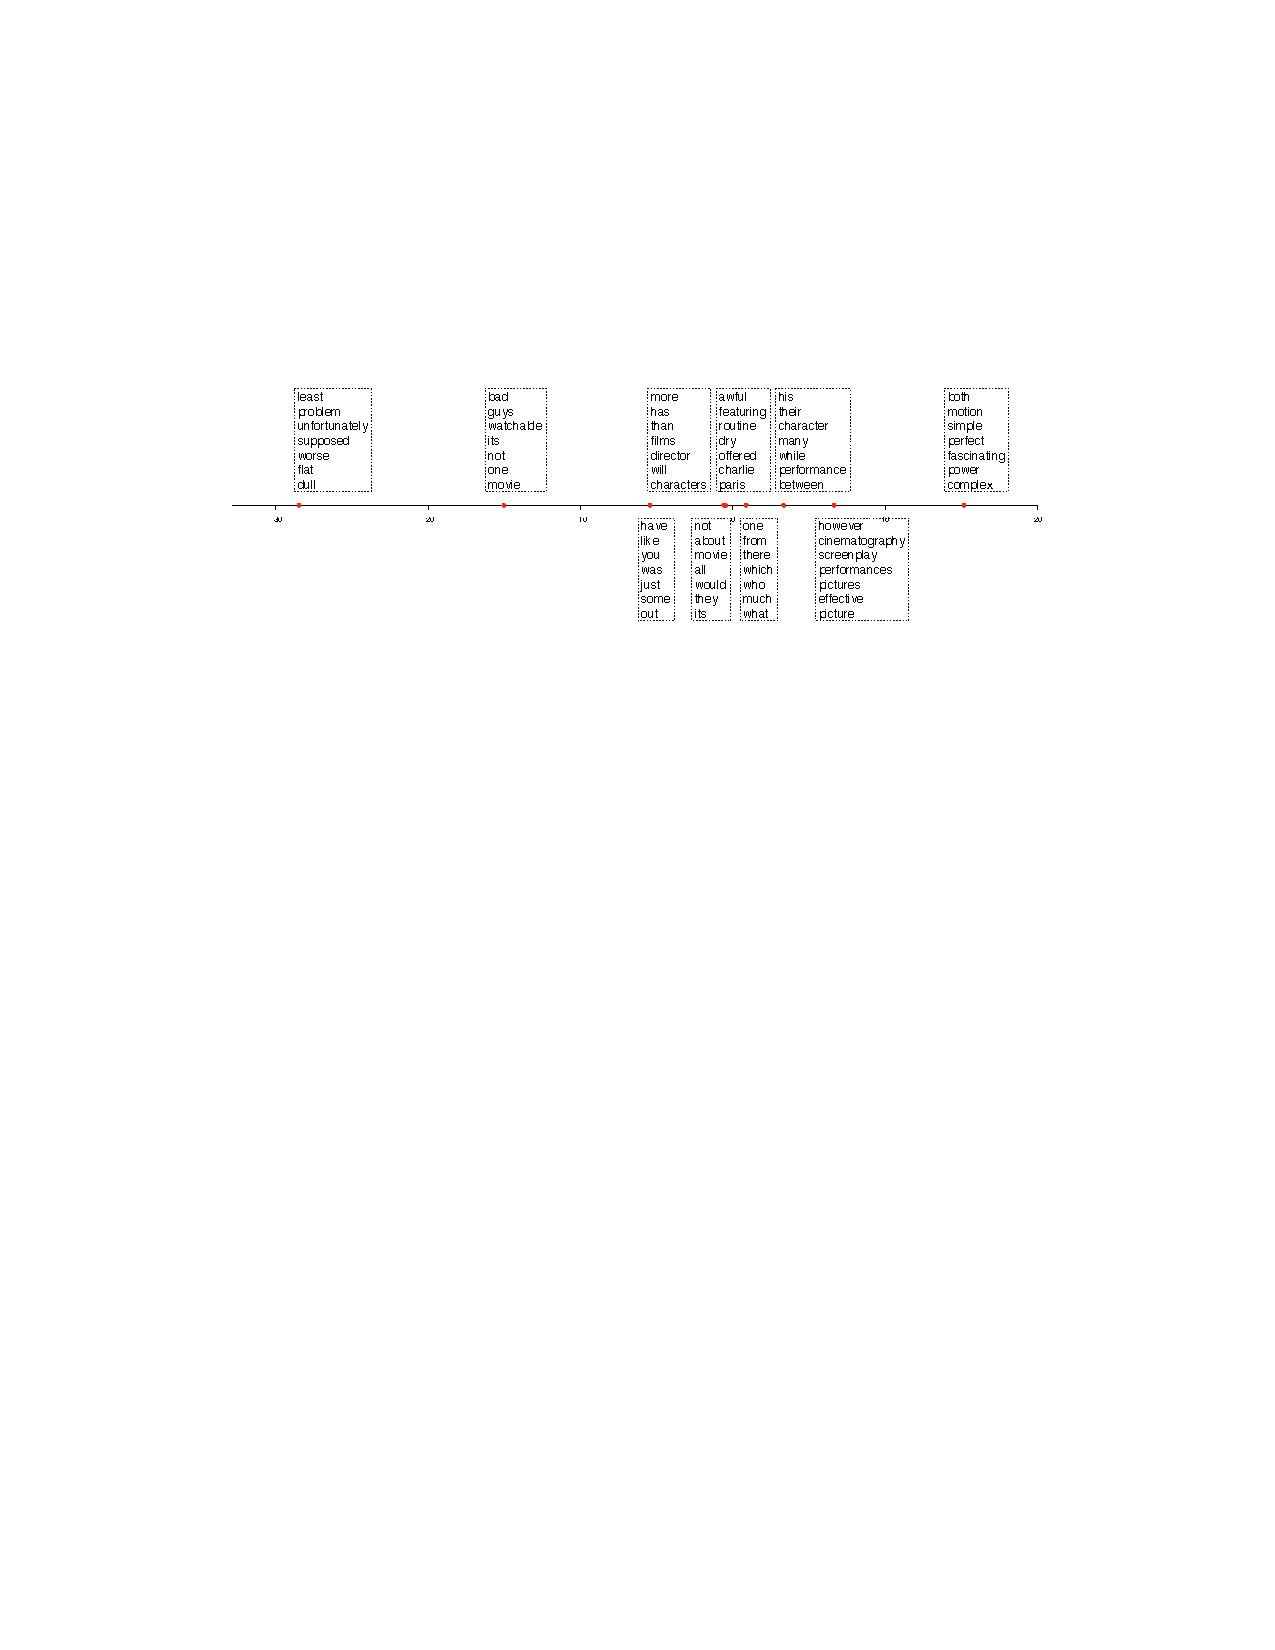
\includegraphics[width=.9\linewidth]{mlslda/slda_example}
	\end{center}

\end{frame}

\frame{
	\frametitle{How to make this multilingual}

	\begin{itemize}
		\item Topic lists provide a layer of abstraction
		\pause
		\item \dots if word lists are consistent across languages
		\item {\bf Holistic}: no component is learned in isolation
	\end{itemize}

	\pause

\begin{center}
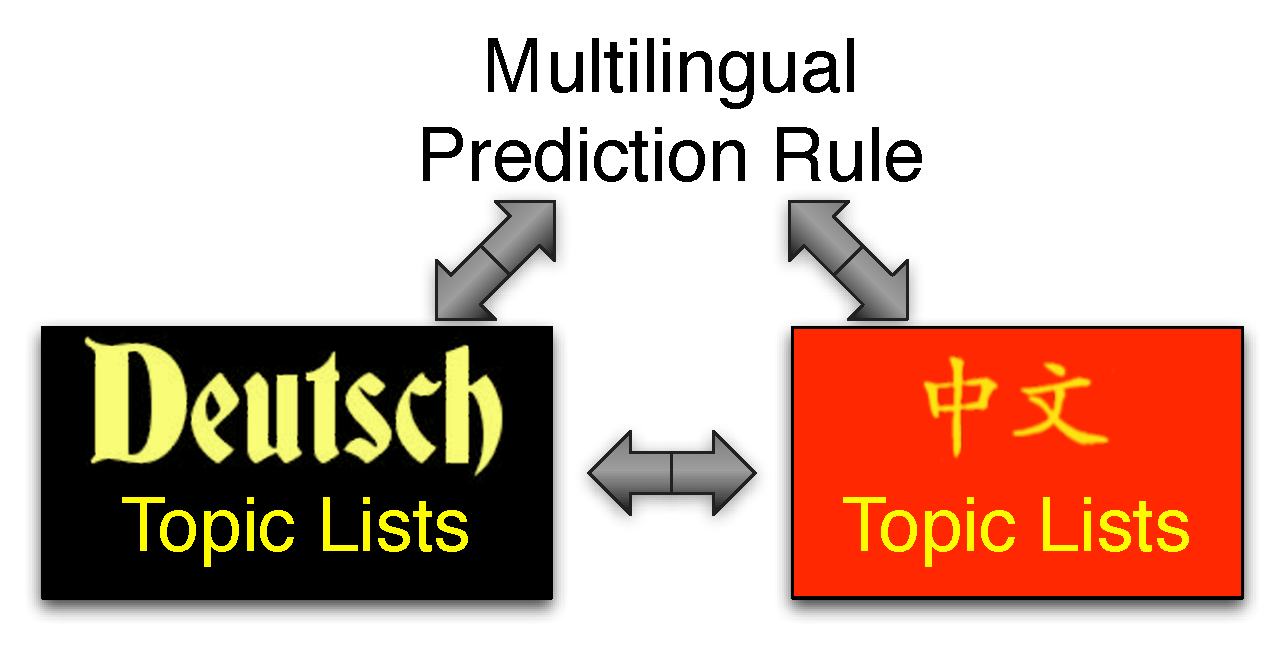
\includegraphics[width=0.6\linewidth]{mlslda/connections}
\end{center}


}

\section{Key Technical Challenge: Correlations Across Languages}



\ifhighlevel

\begin{frame}{Encoding Correlations}

  \begin{itemize}
    \item Statistical NLP typically uses Dirichlet distributions because of conjugacy
   \item Parameter of Dirichlet encode mean and variance
    \pause
    \item But we want correlations!
      \end{itemize}

\begin{center}
  \includegraphics[width=0.85\linewidth]{mlslda/correlations_3}
\end{center}

\end{frame}

\else

\frame {
  \frametitle{Encoding Correlations}

  \begin{itemize}
    \item Statistical NLP typically uses Dirichlet distributions because of conjugacy
    \begin{center}
    	\includegraphics[width=0.5\linewidth]{topic_models/dirichlet_1} \\
    	\includegraphics[width=0.5\linewidth]{topic_models/dirichlet_2}
    \end{center}

    \item Parameter of Dirichlet encode mean and variance
    \pause
    \item But we want correlations!

        \end{itemize}
    \begin{block}{}
    \begin{center}
    \begin{tabular}{ccc}
    	gut & h\v{a}o & good \\
    \end{tabular}
    \end{center}
    \end{block}


}

\frame{
	\frametitle{Encoding Correlations}

\begin{center}
\only<1>{\includegraphics[width=0.85\linewidth]{mlslda/correlations_naive}}
\only<2>{\includegraphics[width=0.85\linewidth]{mlslda/correlations_naive_1}}
\only<3>{\includegraphics[width=0.85\linewidth]{mlslda/correlations_naive_2}}
\only<4>{\includegraphics[width=0.85\linewidth]{mlslda/correlations}}
\only<5>{\includegraphics[width=0.85\linewidth]{mlslda/correlations_1}}
\only<6>{\includegraphics[width=0.85\linewidth]{mlslda/correlations_2}}
\only<7>{\includegraphics[width=0.85\linewidth]{mlslda/correlations_3}}
\end{center}
}

\fi

\section{Sources of Correlation}

\frame
{
  \frametitle{Dictionary}

\begin{columns}
\column{.6\textwidth}

\begin{center}
\includegraphics[width=0.9\linewidth]{mlslda/dictionary}
\end{center}

\column{.4\textwidth}
\begin{block}{}
	\begin{itemize}
		\item CEDICT (Chinese/English) \cite{cedict}
		\item HanDeDict (Chinese/German) \cite{handedict}
		\item Ding (German/English) \cite{richter-08}
	\end{itemize}
\end{block}

\end{columns}

}

\fi

\frame
{
  \frametitle{Multilingual Ontology}

\begin{center}
\includegraphics[width=0.75\linewidth]{mlslda/germanet}
\end{center}

\vspace{-.8cm}

\begin{center}
	\item GermaNet~\cite{hamp-97,kunze-02}
\end{center}

}

%\section{Multilingual Supervised Latent Dirichlet Allocation}

\ifhighlevel

\else

\frame
{
  \frametitle{Generative Model}

\begin{columns}

\column{.4\textwidth}

\begin{block}{}
\begin{enumerate}
	\item For each topic $k = 1 \dots K$, \alert<2>{draw correlated multilingual word distribution $\{{\bm \beta}_k, {\bm \omega}_k, {\bm \phi}_k\}$}
	\item For each document $d$, $\theta_d \sim \mbox{Dir}(\alpha)$
	\begin{enumerate}
	\item $z_{d,n} \sim \mbox{Discrete}(\theta_d)$
	\item \alert<3> {Draw path $\lambda_{d,n}$ through multilingual tree $z_{d,n}$, emit $w_{d,n}$}
	\end{enumerate}
	\item $y_d \sim \mbox{Norm}(\eta^{\top} \bar{z}, \sigma^2)$
\end{enumerate}
\end{block}

\column{.6\textwidth}

\begin{center}
\includegraphics[width=0.9\linewidth]{mlslda/mlslda}
\end{center}

\end{columns}

}

\fi

\iflong

\frame{
	\frametitle{Inference}

	\begin{itemize}
		\item Jointly sample $z$ and path $\lambda$ through multilingual tree

\begin{align}
\textstyle
p(&z_{n} = k, \lambda_{n} = r | {\bm z}_{-n}, {\bm \lambda}_{-n}, w_n, \eta, \sigma, \Theta) = \nonumber \\
& p(y_d | {\bm z}, \eta, \sigma) p(\lambda_{n} = r | z_{n} = k, {\bm \lambda}_{-n}, w_n, {\bm \tau}, {\bm \kappa}, {\bm \pi}) \nonumber \\
& p(z_{n} = k | {\bm z}_{-n}, \alpha). \nonumber
\label{eq:path-topic-sampling}
\end{align}

		\item Collapse out multinomial distributions in tree
		\item Slice sample hyperparameters
		\item After pass of $z$, update $\eta$
	\end{itemize}
}

\fi

\ifsupershortmlslda

\frame{
\frametitle{Multilingual Supervised LDA}
\begin{center}
\includegraphics[width=0.9\linewidth]{mlslda/german_amazon_dict}
\end{center}
}

\else

\begin{comment}
\column{.3\textwidth}
\begin{block}{}
	\begin{enumerate}
		\item For each topic 1 \dots K, draw correlated multilingual word distribution $\{\beta, \omega, \phi\}$
		\item For each document in language:
		\begin{enumerate}
			\item Draw distribution over topics $\theta_d \sim \mbox{Dir}(\alpha)$
			\item For each word $n = 1 \dots d_n$
				\begin{enumerate}
					\item Draw a topic list assignment	$z_n \sim \mbox{Discrete}(\theta_d)$
					\item Draw word $w_n$ from multilingual word distribution $\{{\bm \beta}_{z_n}, {\bm \omega}_{z_n}, {\bm \pi}_{z_n}\}$
				\end{enumerate}
			\item Draw response $y_d \sim \mbox{Norm}(\eta z, \sigma^2)$
		\end{enumerate}
	\end{enumerate}
\end{block}
\column{.7\textwidth}

\end{comment}

\section{Evaluation}


\frame
{
  \frametitle{Evaluation: Learned Topics (Chinese - German)}

\begin{center}
\includegraphics[width=0.9\linewidth]{mlslda/chinese_amazon_dict}
\end{center}

}
\fi

\ifhighlevel

\else

\frame
{
  \frametitle{Evaluation: Learned Topics (English - German)}

\begin{center}
\includegraphics[width=0.9\linewidth]{mlslda/german_amazon_dict}
\end{center}

}

\fi

\frame {

\frametitle{Evaluation: Prediction Accuracy}

\begin{itemize}

\item Take large corpus (6000) of English movie reviews rated from 0-100~\cite{pang-05}
\item Combine them with smaller German corpus (300) rated using same system
\item Compute mean squared error (lower is better) on held out data
\end{itemize}

\begin{center}
\begin{tabular}{ccccc}
Train   & Test & GermaNet     & Dictionary        & Flat \\
\hline
DE      & DE   & 73.8         & 24.8              & 92.2 \\
EN      & DE   & 7.44         & 2.68              & 18.3 \\
EN + DE & DE   & {\bf 1.17}  & {\bf 1.46}        & {\bf 1.39} \\
\end{tabular}
\end{center}

\begin{block}{}
Moral: More data, even in another language, helps
\end{block}

}


\iflong

\frame{
	\frametitle{Related work: Modeling}

    \begin{itemize}
	\item    Alternatives often are difficult (not {\bf conjugate})
        \begin{itemize}
    	\item Logistic normal~\cite{blei-06}
	\item ILP~\cite{ravi-09}
   \end{itemize}
   \item Multilingual topic modeling often assumes parallelism
   \begin{itemize}
   	\item word level~\cite{zhao-06}
	\item document level~\cite{mimno-09}
   \end{itemize}
   \item Richer concept representation~\cite{jagarlamudi-10}
   \item Easier inference~\cite{boyd-graber-09}
   \end{itemize}
}

\frame{
	\frametitle{Related work: Sentiment}
	\begin{itemize}
		\item Gibbs sampling inference for supervised topic model~\cite{blei-07b}
		\item Similar in spirit co-training techniques~\cite{wei-10}
		\item Doesn't rely on translation~\cite{banea-08}
		\item No specialized multilingual sentiment resources~\cite{denecke-08}
	\end{itemize}
}



\frame {

\frametitle{Next Steps}

\begin{itemize}
\item Richer responses
\item More languages
\item Moving beyond bag of words
\item Different structures for knowledge
\item Using human coding as topic seeds
\item Larger corpora
\end{itemize}

}

\fi

\frame{
\frametitle{Takeaway}

\begin{itemize}
\item {\bf Single} model for both languages
\item Requires neither automatic translation nor parallel text
\item Shows flexibility of probabilistic formalism
\end{itemize}

}



